\documentclass[10pt,oneside]{article}

\usepackage{amsmath}
\usepackage{bm}
\usepackage{mathpazo}
\usepackage{graphicx}
\usepackage{enumerate}
\usepackage[x11names, svgnames]{xcolor} % for \definecolor

\usepackage[letterpaper]{geometry}
\geometry{verbose,tmargin=0.25in,bmargin=0.5in,lmargin=1in,rmargin=1.15in}

 \definecolor{saitPurple}{RGB}{112,40,119}
 \definecolor{statsMaroon}{rgb}{0.55, 0, 0}
 \definecolor{saitMaroon}{rgb}{0.55, 0, 0}
 \definecolor{saitRed}{RGB}{224,38,37}
 \definecolor{saitBlue}{rgb}{0, 0.59, 0.85}
 \definecolor{statsDeepBlue}{RGB}{0, 99, 167}
 \definecolor{saitDeepBlue}{RGB}{0, 99, 167}
 \definecolor{LightGrey}{RGB}{200,200,200}
%  \definecolor{boxBG}{RGB}{236, 227, 227}
%  \definecolor{boxBG}{RGB}{242, 233, 223}
\usepackage{xcolor}
\usepackage{cancel}
\usepackage{bm}
\usepackage{graphicx}
\usepackage{hyperref}
\usepackage{adjustbox}
\hypersetup{colorlinks, allcolors=.,urlcolor=structure}
\usepackage{booktabs}  % for top and bottom spacing in table cells, \addlinespace
\usepackage[x11names, svgnames]{xcolor} % for colors in handouts, auto loaded in Beamer?
\usepackage{tikz}
\usetikzlibrary{arrows.meta, math, calc, shadows,bending}
\usetikzlibrary{decorations.markings, decorations.fractals, decorations.text} % for chain, etc.
\usetikzlibrary{intersections}
\usepackage{pgfmath}
\usepackage{ifthen}
\usepgfmodule{oo}
\usetikzlibrary{shadings}
% \usetikzlibrary{decorations.shapes}
\usepackage[many]{tcolorbox}
\tcbuselibrary{skins} % for image boxes
\usepackage[absolute,overlay,showboxes]{textpos}
% \usepackage{textpos}
% \textblockorigin{0.0cm}{0.0cm}  %start all at upper left corner
\TPshowboxesfalse

\newcommand\lb{\linebreak}
\newcommand\Ra{\Rightarrow}
\newcommand\cd{\!\cdot\!}
\newcommand\x{\!\times\!}
\newcommand\pars{\par\smallskip}
\newcommand\parm{\par\medskip}
\newcommand\parb{\par\bigskip}
\renewcommand{\deg}{^\circ}

% counter for resuming enumerated list numbers
\newcounter{resumeenumi}
\newcommand{\suspend}{\setcounter{resumeenumi}{\theenumi}}
\newcommand{\resume}{\setcounter{enumi}{\theresumeenumi}}



% https://tex.stackexchange.com/questions/33703/extract-x-y-coordinate-of-an-arbitrary-point-in-tikz
\makeatletter
\providecommand{\gettikzxy}[3]{%
	\tikz@scan@one@point\pgfutil@firstofone#1\relax
	\edef#2{\the\pgf@x}%
	\edef#3{\the\pgf@y}%
}
\makeatother

\makeatletter
\newcommand{\verbatimfont}[1]{\def\verbatim@font{#1}}%
\makeatother

%%%%%%%%%%%%%%%%%%%%%%%%%%%%%%%%%%%%%%%%%%%%%%%%%%%%%%%%%%%%%%%%%%%%%%%%%%%%%%%%


% \newcommand{\tb}[4][0.8]{
% 	\begin{textblock*}{#1}(#2, #3)
% 		\raggedright
% 		#4
% 	\end{textblock*}
% }

% \def\tb

\newtcolorbox{statsbox}[2][] { 
  colback=white,
  colbacktitle=structure,
  colframe=structure,
  coltitle=white,  
  top=0.25cm,
	bottom=0.125cm,
	left=0mm,
	right=0mm,
  % fonttitle=\itshape\rmfamily,
  halign=flush left, 
  enhanced,
  drop fuzzy shadow,
  attach boxed title to top left={xshift=3.5mm, yshift=-2mm},
  title={#2}, #1}
\newtcolorbox{redbox}{colback=white, colframe=structure, enhanced, drop fuzzy shadow}
\newtcolorbox{titledbox}[1]{colback=white,colframe=structure,title={#1}}
\newtcbox{\tcb}[1][]{colback=white,boxsep=0pt,top=0.5cm,bottom=0.5cm,left=0.5cm,
		right=0.5cm, colframe=structure,  enhanced, drop fuzzy shadow, #1}
\newtcbox{\tcbfig}[1][1]{colback=white,boxsep=0pt,top=0.5cm,bottom=0.5cm,left=0.5cm,
		right=0.5cm, colframe=structure,  enhanced, drop fuzzy shadow, #1}
% tcb title
\newtcbox{\tcbt}[2][]{colback=white,boxsep=0pt,top=5pt,bottom=5pt,left=5pt,
		right=5pt, colframe=structure, enhanced, drop fuzzy shadow,  title={#2}, #1}
% tcb left title
\newtcbox{\tcbtl}[2][]{ colback=white,
  colbacktitle=structure,
  colframe=structure,
  coltitle=white,  
  top=0.25cm,
	bottom=0.125cm,
	left=0mm,
	right=0mm,
  % fonttitle=\bfseries,
  halign=flush left, 
  enhanced,
  drop fuzzy shadow,
  attach boxed title to top left={xshift=3.5mm, yshift=-2mm}, 
	title={#2}, #1}

\newtcbtheorem{myexam}{Example}%
{
	enhanced,
	colback=white,
	colframe=structure,
	% fonttitle=\bfseries,
	fonttitle=\itshape\rmfamily,
	drop fuzzy shadow,
	%description font=\mdseries\itshape,
	attach boxed title to top left={yshift=-2mm, xshift=5mm},
	colbacktitle=structure
	}{exam}% then \pageref{exer:theoexample} references the theo

% \newcommand{\myexample}[2][red]{
% 	% \tcb\tcbset{theostyle/.style={colframe=red,colbacktitle=yellow}}
% 	\begin{myexam}{}{}
% 		#2
% 	\end{myexam}
% 	% \tcbset{colframe=structure,colbacktitle=structure}
% }

\newtcbtheorem{myexer}{Exercise}%
{
	enhanced,
	colback=white,
	colframe=structure,
	% fonttitle=\bfseries,
	drop fuzzy shadow,
	fonttitle=\itshape\rmfamily,
	% description font=\mdseries\itshape,
	attach boxed title to top left={yshift=-2mm, xshift=5mm},
	colbacktitle=structure
	}{exer}



\newcommand{\mini}[2][0.8]{
	\begin{minipage}[c]{#1\columnwidth}
		\raggedright
		#2
	\end{minipage}
}
\newcommand{\minit}[2][0.8]{
	\begin{minipage}[t]{#1\columnwidth}
		% \raggedright
		#2
	\end{minipage}
}

% centered minipage with text \raggedright
%\cmini[width]{content}
\newcommand{\cmini}[2][0.8]{
	\begin{center}
		\begin{minipage}{#1\columnwidth}
			\raggedright
			#2
		\end{minipage}
	\end{center}
}

\newcommand{\fig}[2][1]{% scaled graphic
	\includegraphics[scale=#1]{#2}
}

% centred framed box black border
%\cbox[width]{content}
\newcommand{\cbox}[2][1]{% framed centered color box
	\setlength\fboxsep{5mm}
	\setlength\fboxrule{.2 mm}
	\begin{center}
		\fcolorbox{black}{white}{
			\vspace{-0.5cm}
			\begin{minipage}{#1\columnwidth}
				\raggedright
				#2
			\end{minipage}
		}
	\end{center}
	\setlength\fboxsep{0cm}
}

\newcommand{\ccbox}[4][1]{% framed centered color box
	\setlength\fboxsep{5mm}
	\setlength\fboxrule{.2 mm}
	\begin{center}
		\fcolorbox{#2}{#3}{
			% \vspace{-0.5cm}
			\begin{minipage}{#1\columnwidth}
				\vspace{-0.25cm}
				\raggedright				
				#4
				\vspace{-0.325cm}
			\end{minipage}
		}
	\end{center}
	\setlength\fboxsep{0cm}
}

\newcommand{\cfig}[2][1]{% centred, scaled graphic
	\begin{center}
		% \fcolorbox{structure}{white}{
		\tcbincludegraphics{
			\includegraphics[scale=#1]{#2}
		}
	\end{center}
}

% figure with tight border for photos
% \cfigb[saitMaroon]{borderwidth with unit}{scale}{image}
\newcommand{\stcsfig}[2][1]{
	% \usepackage{adjustbox}
	% \setlength{\fboxrule}{1pt}
	\begin{center}
		\tcbincludegraphics[width=#1\textwidth, boxrule=2pt, top=-3pt, right=-3pt, left=-3pt, bottom=-3pt,colframe=structure, sharp corners, enhanced, drop fuzzy shadow]{#2}
	\end{center}
}






%\Member{startpt}{endpt}{outer fill color}{inner fill color}{stroke}{height}{radius}{linewidth}
\providecommand{\Member}[8]{
  % name the points
  \coordinate(start) at (#1);
  \coordinate(end) at (#2);
  \edef\ofill{#3}%
  \edef\ifill{#4}%
  \edef\stroke{#5}%
  \edef\height{#6} % cm
  \edef\radius{#7} % cm
  \edef\linewidth{#8} % mm

  \coordinate(delta) at ($ (end)-(start) $);
  \gettikzxy{(delta)}{\dx}{\dy}
  \gettikzxy{(start)}{\sx}{\sy}
  \pgfmathparse{veclen(\dx, \dy)} \let\length\pgfmathresult

  \pgfmathparse{\dx==0}%
  % \ifnum low-level TeX for integers
  \ifnum\pgfmathresult=1 % \dx == 0
    \pgfmathsetmacro{\rot}{\dy > 0 ? 90 : -90}
  \else
    \pgfmathsetmacro{\rot}{\dx > 0 ? atan(\dy / \dx) : 180 + atan(\dy / \dx)}
  \fi

  
   
  \shadedraw[transform canvas = { rotate around = {\rot:(\sx,\sy)}}, line width = \linewidth, rounded corners = \radius mm, top color = \ofill, bottom color = \ofill, middle color = \ifill, draw = \stroke] ($ (start)+(-0.5*\height, 0.5*\height) $) -- ++(\height cm +\length pt, 0 ) -- ++(0, -\height) -- ++ (-\height cm -\length pt, 0) -- cycle;


  \shadedraw[ball color = \ofill!50!\ifill, draw = \stroke] (start) circle (\height/8);
  \shadedraw[ball color = \ofill!50!\ifill, draw = \stroke] (end) circle (\height/8);
  %  \pgfresetboundingbox

  
  


}

%\Member{startpt}{endpt}{outer fill color}{inner fill color}{stroke}{height}{radius}{linewidth}
\providecommand{\Meme}[8]{
  \coordinate(start) at (#1);
  \coordinate(end) at (#2);
  \edef\ofill{#3}%
  \edef\ifill{#4}%
  \edef\stroke{#5}%
  \edef\height{#6} % cm
  \edef\radius{#7} % cm, should be half \height or less
  \edef\linewidth{#8} % mm

  


  \coordinate(delta) at ($ (end)-(start) $);
  \gettikzxy{(delta)}{\dx}{\dy}
  \gettikzxy{(start)}{\sx}{\sy}
  \gettikzxy{(end)}{\ex}{\ey}
  \pgfmathparse{veclen(\dx, \dy)} \let\length\pgfmathresult
  \pgfmathparse{\height*28.435} \let\heightpt\pgfmathresult
  \pgfmathparse{\heightpt/\length} \let\ratio\pgfmathresult
  \pgfmathparse{1/\ratio} \let\inverse\pgfmathresult
  

  \pgfmathparse{\dx==0}%
  % \ifnum low-level TeX for integers
  \ifnum\pgfmathresult=1 % \dx == 0
    \pgfmathsetmacro{\rot}{\dy > 0 ? 90 : -90}
  \else
    \pgfmathsetmacro{\rot}{\dx > 0 ? atan(\dy / \dx) : 180 + atan(\dy / \dx)}
  \fi

  \pgfmathparse{round(mod(abs(\rot),90))} \let\tmp\pgfmathresult
  \pgfmathsetmacro{\rotmod}{\tmp>45?90-\tmp:\tmp}
  \pgfmathparse{(0.007*\rotmod-0.315)/45+1.017} \let\rotfudge\pgfmathresult

  % \pgfmathparse{mod(abs(\rot),90)} \let\moded\pgfmathresult
  % \ifthenelse{\moded>45}{
  %   \pgfmathparse{90-\moded} \let\rotmod\pgfmathresult    
  % }{
  %   \pgfmathparse{div(\moded,1)} \let\rotmod\pgfmathresult   
  % }


  
  \pgfmathparse{1+3.62/(1+(\inverse/0.714)^1.69)} \let\fudge\pgfmathresult
  \pgfmathparse{50*(1-\ratio)*\fudge*\rotfudge} \let\colorstop\pgfmathresult
  \pgfmathparse{(100-\colorstop)} \let\colorstoptwo\pgfmathresult

  \pgfdeclareverticalshading{myshade}{100bp}{%
					color(0bp)=(\ofill);
					% color(\colorstop bp)=(\ofill);
					color(\colorstop bp)=(\ofill);
					color(50 bp)=(\ifill);
					color(\colorstoptwo bp)=(\ofill);
					color(100bp)=(\ofill)}

  % \tikzset{shading=myshade}

  \begin{scope}[rotate around = {\rot:(start)}, rounded corners = \radius cm, shading angle=\rot]
    \begin{scope} 
      \path[clip]($ (start)+(-0.5*\height, 0.5*\height cm) $) rectangle +(\length pt+\height cm, -\height);
      \shade[shading=myshade] ($ (start)+(-0.5*\height, 0.5*\length pt) $) rectangle +(\length pt+\height cm, -\length pt);
    \end{scope}
  \draw[line width=\linewidth, \stroke] ($ (start)+(-0.5*\height, 0.5*\height cm) $) rectangle +(\length pt+\height cm, -\height);

  % \shadedraw[top color=\ofill, bottom color=\ofill, middle color=\ifill, rotate around = {\rot:(start)}, draw=\stroke, rounded corners = \radius cm, , shading angle=\rot] ($ (start)+(-0.5*\height cm, 0.5*\length pt) $) rectangle +(\length pt+\height cm, -\length pt);
  \end{scope}

  % \pgfresetboundingbox


  % \node[orange] at (0,-1) {rot: \rot};  
  % \node[orange] at (0,-1.5) {rotmod: \rotmod};  
  % \node[orange] at (0,-2) {rotfudge: \rotfudge};  
  % \node[orange] at (-2,-1) {stop2: \colorstoptwo};  
  % \node[orange] at (-2,-1.5) {l/h: \inverse};  
  % \node[orange] at (-2,-2) {fudge: \fudge};  

 
  
  \shade[ball color=\ofill] (start) circle (\height/4);
  \shade[ball color=\ofill] (end) circle (\height/4);

  % \draw(current bounding box.south west) rectangle (current bounding box.north east);


}

\newcommand{\PC}[6][0]{%
  \edef\lrotate{#1}%
  \edef\lpin{#2}%
  \edef\lfill{#3}%
  \edef\ldraw{#4}%
  \edef\lscale{#5}%
  \edef\lwidth{#6}%
  \edef\h{1}%
  \edef\r{0.3}%
  \begin{scope}[scale=\lscale, rotate=\lrotate]
	\filldraw[draw=\ldraw, fill=\lfill, line width=\lwidth mm] ($ (\lpin) + (0.201*\h+1.0353*\r ,-0.75*\h) $) -- ++(105: 0.77646*\h+0.26795*\r) arc (15:165:\r) -- ++(-105:0.77646*\h+0.26795*\r) -- cycle;

	\shadedraw[ball color=\lfill, draw=\ldraw, line width = \lwidth mm] (\lpin) circle (1.5mm);

	\filldraw[rounded corners=\lscale pt, draw=\ldraw, fill=\lfill, line width=\lwidth mm] ($ (\lpin) - (1,1) $) rectangle +(2,0.25);
  \end{scope}%
}



% !TEX root = ../../Beamer/statikz/statikz.tex


\newcommand{\EyeConnection}[6][0]{
	\def\lrotate{#1};
	\def\lpin{#2}
	\def\lfill{#3}
	\def\ldraw{#4}
	\def\lscale{#5}
	\def\lwidth{#6}
	\def\h{1}
	\def\r{0.3}
	\begin{scope}[scale=\lscale, rotate=\lrotate]
		\filldraw[draw=\ldraw, fill=\lfill, line width=\lwidth pt] ($(\lpin) + (0.201*\h+1.0353*\r ,-0.75*\h)$) -- ++(105: 0.77646*\h+0.26795*\r) arc (15:165:\r) -- ++(-105:0.77646*\h+0.26795*\r) -- cycle;

		\fill[outer color=\lfill, middle color=red, inner color=black, line width = \lwidth pt] (\lpin) circle (2.5mm);
		\filldraw[fill=white, draw=\ldraw, line width = \lwidth pt] (\lpin) circle (1.25mm);

		\filldraw[rounded corners=\lscale pt, draw=\ldraw, fill=\lfill, line width=\lwidth pt] ($ (\lpin) - (1,1) $) rectangle +(2,0.25);
	\end{scope}
}

% !TEX root = ../Beamer/02ForceVectors/02ForceVectors.tex


\newcommand{\EyeBolt}[6][0]{
	\def\lrotate{#1};
	\def\lpin{#2}
	\def\lfill{#3}
	\def\ldraw{#4}
	\def\lscale{#5}
	\def\lwidth{#6}
	%\def\h{1.5}
	\def\r{0.3}
	\begin{scope}[scale=\lscale, rotate=\lrotate]
		\filldraw[draw=\ldraw, fill=\lfill, line width=\lwidth pt] ($(\lpin) + (-0.7,-1.25)$) arc(180:90:.2) -- ++(0.05,0)arc(-90:0:0.2) -- ++(0.05,0.65)arc(225:-45:0.28284)-- ++(0.05,-.65)arc(180:270:.2)-- ++(0.05,0)arc(90:0:0.2) -- cycle;
		\fill[outer color=\lfill, inner color=black, line width = 0] (\lpin) circle (2.25mm);
		\filldraw[fill=white, draw=\ldraw, line width = \lwidth pt] (\lpin) circle (1.25mm);

		\begin{scope}[even odd rule]
			\fill[\lfill] (\lpin) circle (2.5mm)
			(\lpin) circle (2.125mm);
		\end{scope}

		\filldraw[rounded corners=\lscale pt, draw=\ldraw, fill=\lfill, line width=\lwidth pt] ($ (\lpin) - (1,1.5) $) rectangle +(2,0.25);
	\end{scope}
}

\input{../../includes/Skywalker.tex}

\newcommand{\PulleyC}[8][0]{
	\def\rotate{#1};
	\def\pin{#2}
	\def\lfill{#3}
	\def\ldraw{#4}
	\def\len{#5}
	\def\wid{#6}
	\def\lscale{#7};
	\def\lwidth{#8};
	\def\h{1}
	\def\r{0.35}
	\def\rr{0.675}
	\begin{scope}[scale=\lscale, rotate=\rotate]

		
		
		\filldraw[draw=\ldraw, fill=\lfill, line width=\lwidth mm] (\pin) circle (\h*\rr cm);
		
		\filldraw[draw=\ldraw, fill=\lfill!70!black, line width=\lwidth mm] (\pin) circle (\h*\rr*0.75 cm);

		\filldraw[ draw=\ldraw, fill=\lfill, line width = \lwidth mm] ($(\pin) + (-\wid,0) $) arc(180:0:\wid) -- ++(0,-\len) arc(0:-180:\wid) -- cycle;		

		% \shadedraw[fill=\lfill, line width = \lwidth pt, draw=\lfill!80!black] (\pin) circle (\h mm);
		\shadedraw[ball color=\lfill, draw=\ldraw, line width = \lwidth mm] (\pin) circle (2*\h*\rr mm);
		\shadedraw[ball color=\lfill, draw=\ldraw, line width = \lwidth mm] ($ (\pin)+(0,-\len) $) circle (2*\h*\rr mm);

		
	\end{scope}
}

% !TEX root = ../Beamer/statikz/statikz.tex

% \Pulley[rotation]{A}{wheel color}{support color}{scale}{line width}
\newcommand{\Pulley}[6][0]{
	\def\lrotate{#1};
	\def\lpin{#2}
	\def\lfill{#3}
	\def\ldraw{#4}
	\def\lscale{#5}
	\def\lwidth{#6}
	\def\h{1}
	\def\r{0.3}
	\def\rr{0.5}
	\begin{scope}[scale=\lscale, rotate=\lrotate]

		\filldraw[draw=\ldraw, fill=\lfill, line width=\lwidth mm] (\lpin) circle (\h*\rr cm);

		\filldraw[draw=\ldraw, fill=\lfill, line width=\lwidth mm] ($(\lpin) + (0.201*\h+1.0353*\r ,-0.75*\h)$) -- ++(105: 0.77646*\h+0.26795*\r) arc (15:165:\r) -- ++(-105:0.77646*\h+0.26795*\r) -- cycle;

		\shadedraw[ball color=\lfill, draw=\ldraw, line width = \lwidth mm] (\lpin) circle (2*\h*\rr mm);

		\filldraw[rounded corners=\lscale pt, draw=\ldraw, fill=\lfill, line width=\lwidth mm] ($ (\lpin) - (1,1) $) rectangle +(2,0.25);
	\end{scope}
}

% !TEX root = ../Beamer/statikz/statikz.tex

% \Ring{A}{outer color}{inner color}{outer radius}{inner radius}{line width}
\newcommand{\Ring}[6]{
	\def\lpin{#1}
	\def\lfill{#2}
	\def\ldraw{#3}
	\def\outerr{#4}
	\def\innerr{#5}
	\def\lwidth{#6}

	\begin{scope}

		\makeatletter
		\providecommand{\gettikzxy}[3]{%
			\tikz@scan@one@point\pgfutil@firstofone#1\relax
			\edef#2{\the\pgf@x}%
			\edef#3{\the\pgf@y}%
		}
		\makeatother

		\gettikzxy{(\lpin)}{\cx}{\cy}
		\pgfdeclareradialshading{ring}{\pgfpoint{0cm}{0cm}}
		{
			color(0cm)=(black);
			color(0.5cm)=(\lfill);
			color(.65cm)=(\ldraw);
			color(1cm)=(\lfill)
		}
		% \pgfuseshading{ring}



	\end{scope}


\begin{scope}[even odd rule]
	% \draw (\lpin) circle (\innerr);
	\filldraw[shading=ring, fill=\lfill, draw=\ldraw, line width=\lwidth] (\lpin) circle (\outerr cm)
		(\lpin) circle (\innerr);
		\draw[black, line width = \lwidth mm] (\lpin) circle (\innerr cm);
		\draw[black, line width = \lwidth mm] (\lpin) circle (\outerr cm);
\end{scope}


}


% https://tex.stackexchange.com/questions/731957/how-to-supress-missing-character-there-is-no-u003b-in-font-nullfont
\tracinglostchars=1

\hfuzz=150pt
\setlength{\parindent}{0pt}
\def\scale{1}

\begin{document}

%%%%%%%%%%%%%%%%%%%%%%%%%%%%%%%%%%%%%%%%%%%%%%%%%%%%%%%%%%%%%%%%%%%%%%%%%%%%%%%%%%%%%%%%%%%%%%%%%%%%
% page 1
%%%%%%%%%%%%%%%%%%%%%%%%%%%%%%%%%%%%%%%%%%%%%%%%%%%%%%%%%%%%%%%%%%%%%%%%%%%%%%%%%%%%%%%%%%%%%%%%%%%%

\begin{textblock*}{7.25in}(1in, 0.4in)
	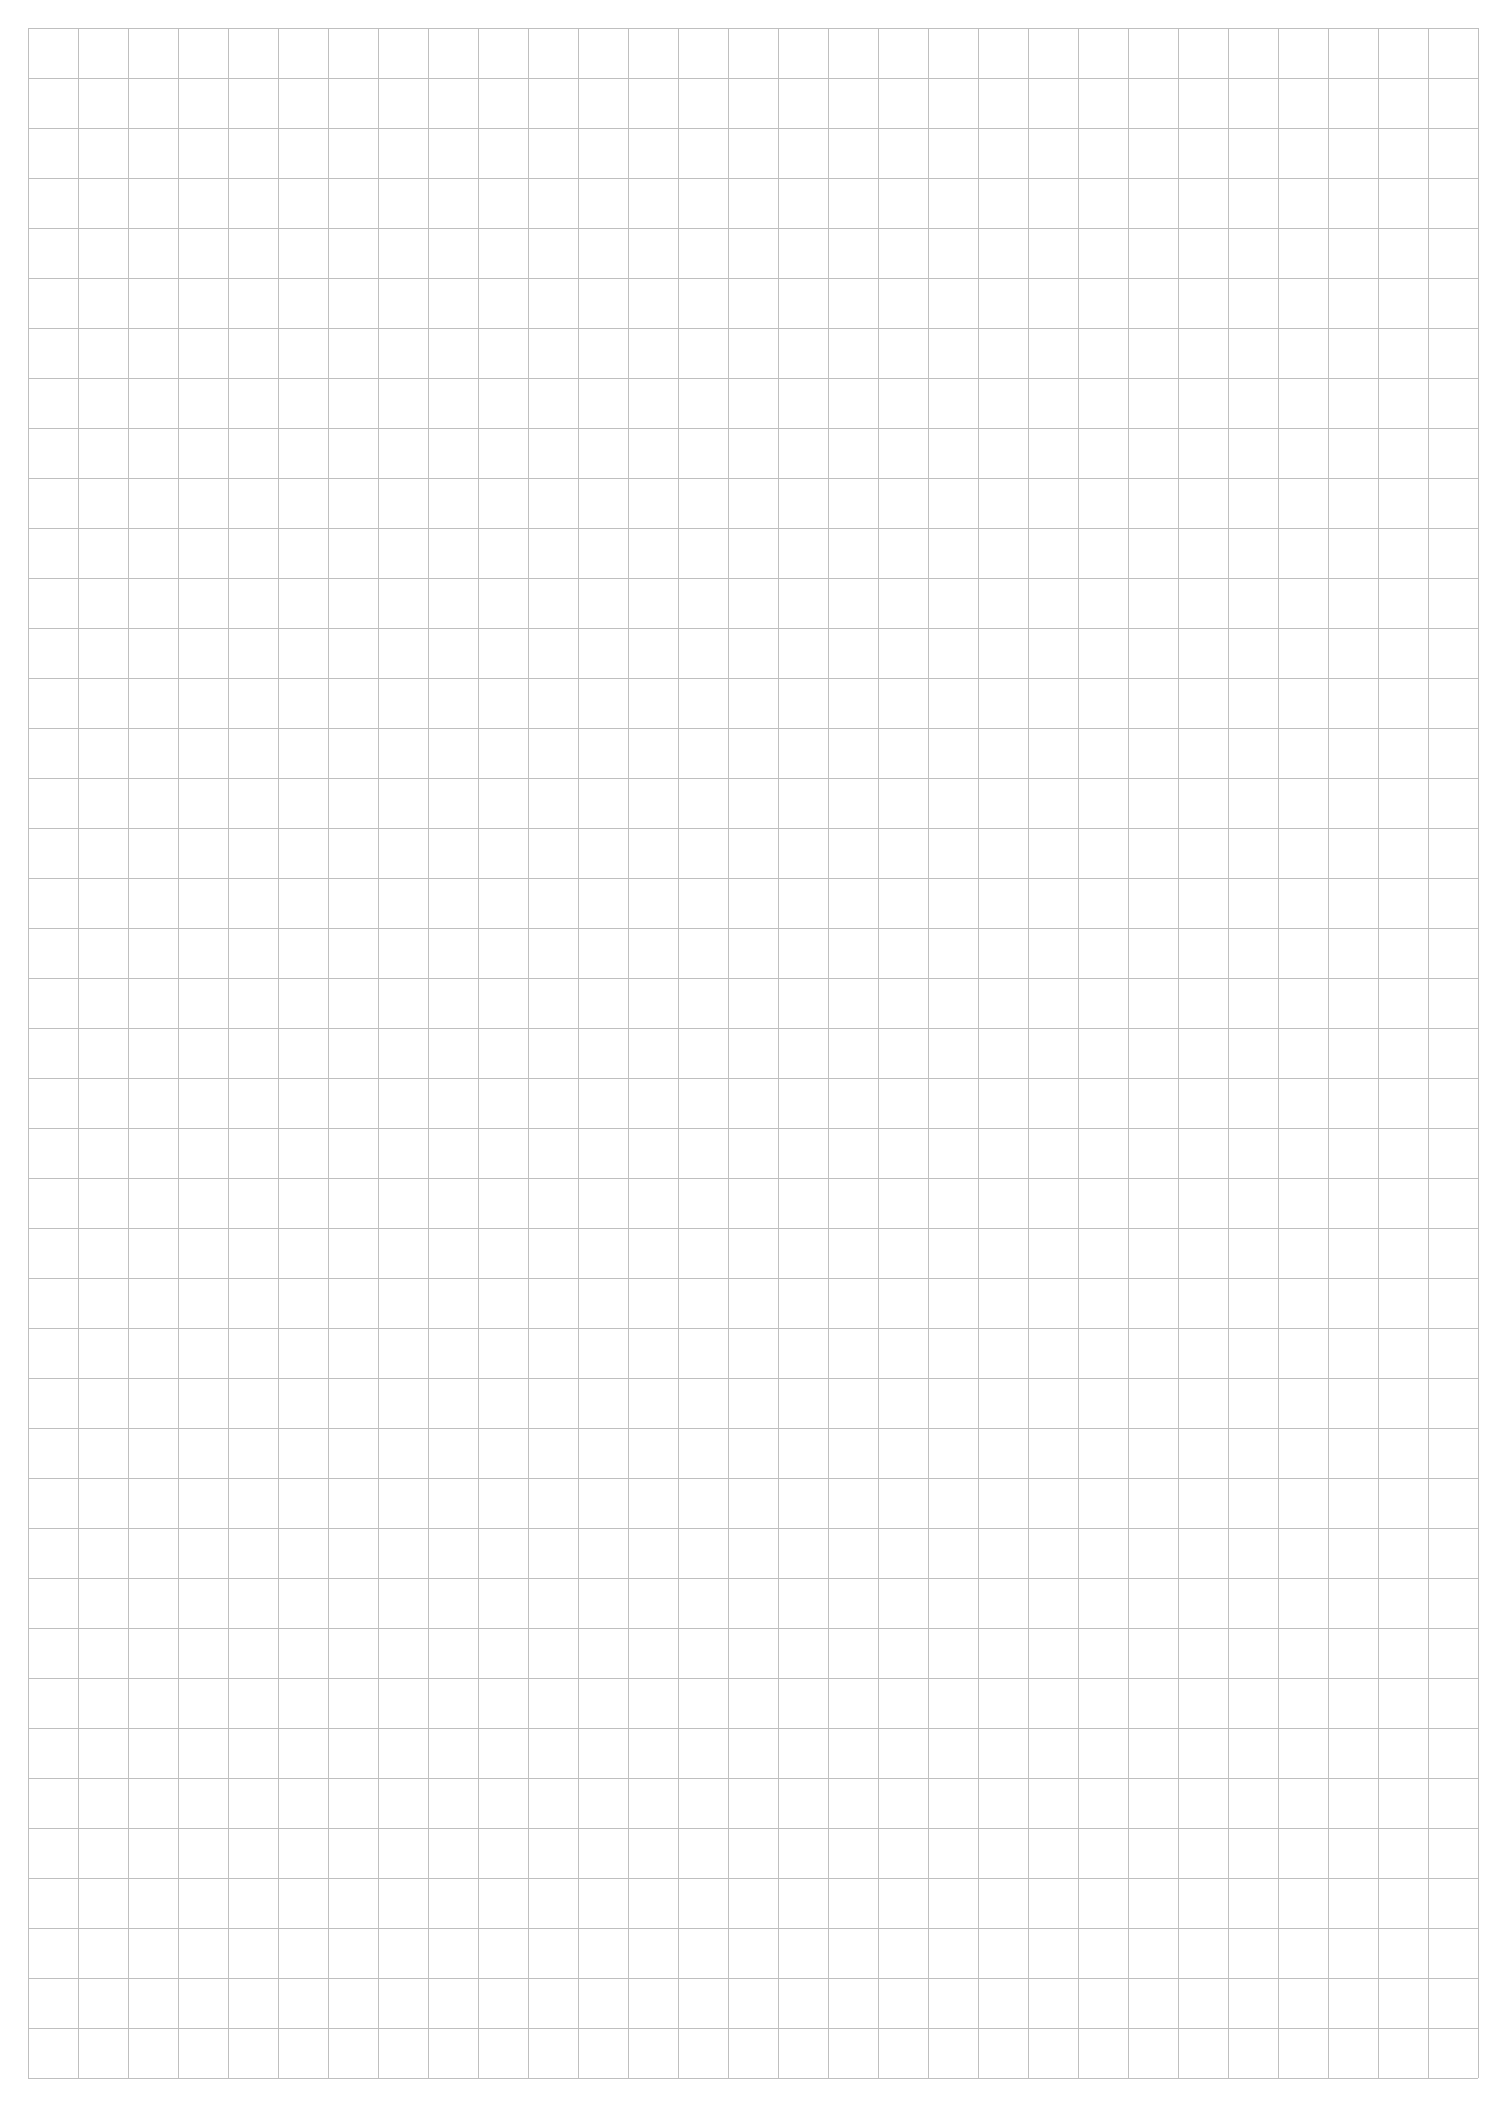
\begin{tikzpicture}[line width=0.1mm]
		\draw[color=gray!50, step=0.25in] (0,0) grid +(7.25in,10.25in);
	\end{tikzpicture}
\end{textblock*}


\begin{textblock*}{6.775in}(1in, 0.225in)
  \cbox{
    \centering\huge
    \textbf{Engineering Statics - 03 Equilibrium of a Particle / Concurrent Forces Handout}
  }
\end{textblock*}

\begin{textblock*}{2.5in}(1in, 1.25in)
	\cbox{
		\underline{Exercise 1} \parm
		The trolley can move freely along the horizontal beam on frictionless rollers. Currently, it is in equilibrium. Determine the reaction at A..
		\parb
		\centering
		\scalebox{0.875}{
			
			\scalebox{.8}{
				\centering
				\tikz[scale=\scale]{
	\coordinate (O) at (0,0);
	\coordinate (A) at (-0.75,0);
	\coordinate (B) at ($ (A)+(-60:1.5) $);
	\coordinate (C) at ($ (A)+(1.5,0)$);


  \fill[Gray!50] ($ (A)+(-3,-0.35) $) rectangle +(7.5,1.5);
  \draw[Black, line width=1mm] ($ (A)+(-3,-0.4) $) -- +(7.5,0);
  \draw[Black, line width=1mm] ($ (A)+(-3,+1.1) $) -- +(7.5,0);
	
  \filldraw[Black] (A) circle (0.35cm);
  \filldraw[Black] (C) circle (0.35cm);
  \filldraw[White] (A) circle (0.3cm);
  \filldraw[White] (C) circle (0.3cm);
		
	\filldraw[fill=Ivory3!60, rounded corners=0.35cm] ($ (A)+(150:0.4cm) $) -- ($ (C)+(30:0.4cm) $) -- ($ (B)+(0,-0.4cm) $) -- cycle;

  \draw[Black, line width = 0.75mm, -latex] (B) -- +(-30:2.5) node[right] {$1260\,$N};
  \draw[Black, line width = 0.75mm, -latex] (B) -- +(220:2.5) node[left] {$P$};

	\shadedraw[ball color=Gray ] (A) circle (0.1cm);% node[left]{A};
	\shadedraw[ball color=Gray ] (B) circle (0.1cm) ;%node[right]{B};
	\shadedraw[ball color=Gray ] (C) circle (0.1cm);% node[below]{C};

  \draw[thin, gray] ($ (B)+(0,-0.325) $) -- +(0,-1.5);

  \draw[latex-latex] ($ (B)+(-30:1.5) $) arc (-30:-90:1.5) node[fill=white, midway, inner sep=0.25mm] {$ 58\deg $};
  \draw[latex-latex] ($ (B)+(-90:1.5) $) arc (-90:-140:1.5) node[fill=white, midway, inner sep=0.25mm] {$ 47\deg $};

  \node at ($ (B)+(0,0.3) $) {\large $ A $};


}
			}			
		}
	}
\end{textblock*}


%%%%%%%%%%%%%%%%%%%%%%%%%%%%%%%%%%%%%%%%%%%%%%%%%%%%%%%%%%%%%%%%%%%%%%%%%%%%%%%%%%%%%%%%%%%%%%%%%%%%
% page 2 
%%%%%%%%%%%%%%%%%%%%%%%%%%%%%%%%%%%%%%%%%%%%%%%%%%%%%%%%%%%%%%%%%%%%%%%%%%%%%%%%%%%%%%%%%%%%%%%%%%%%

~\newpage
\begin{textblock*}{7.25in}(1in, 0.4in)
	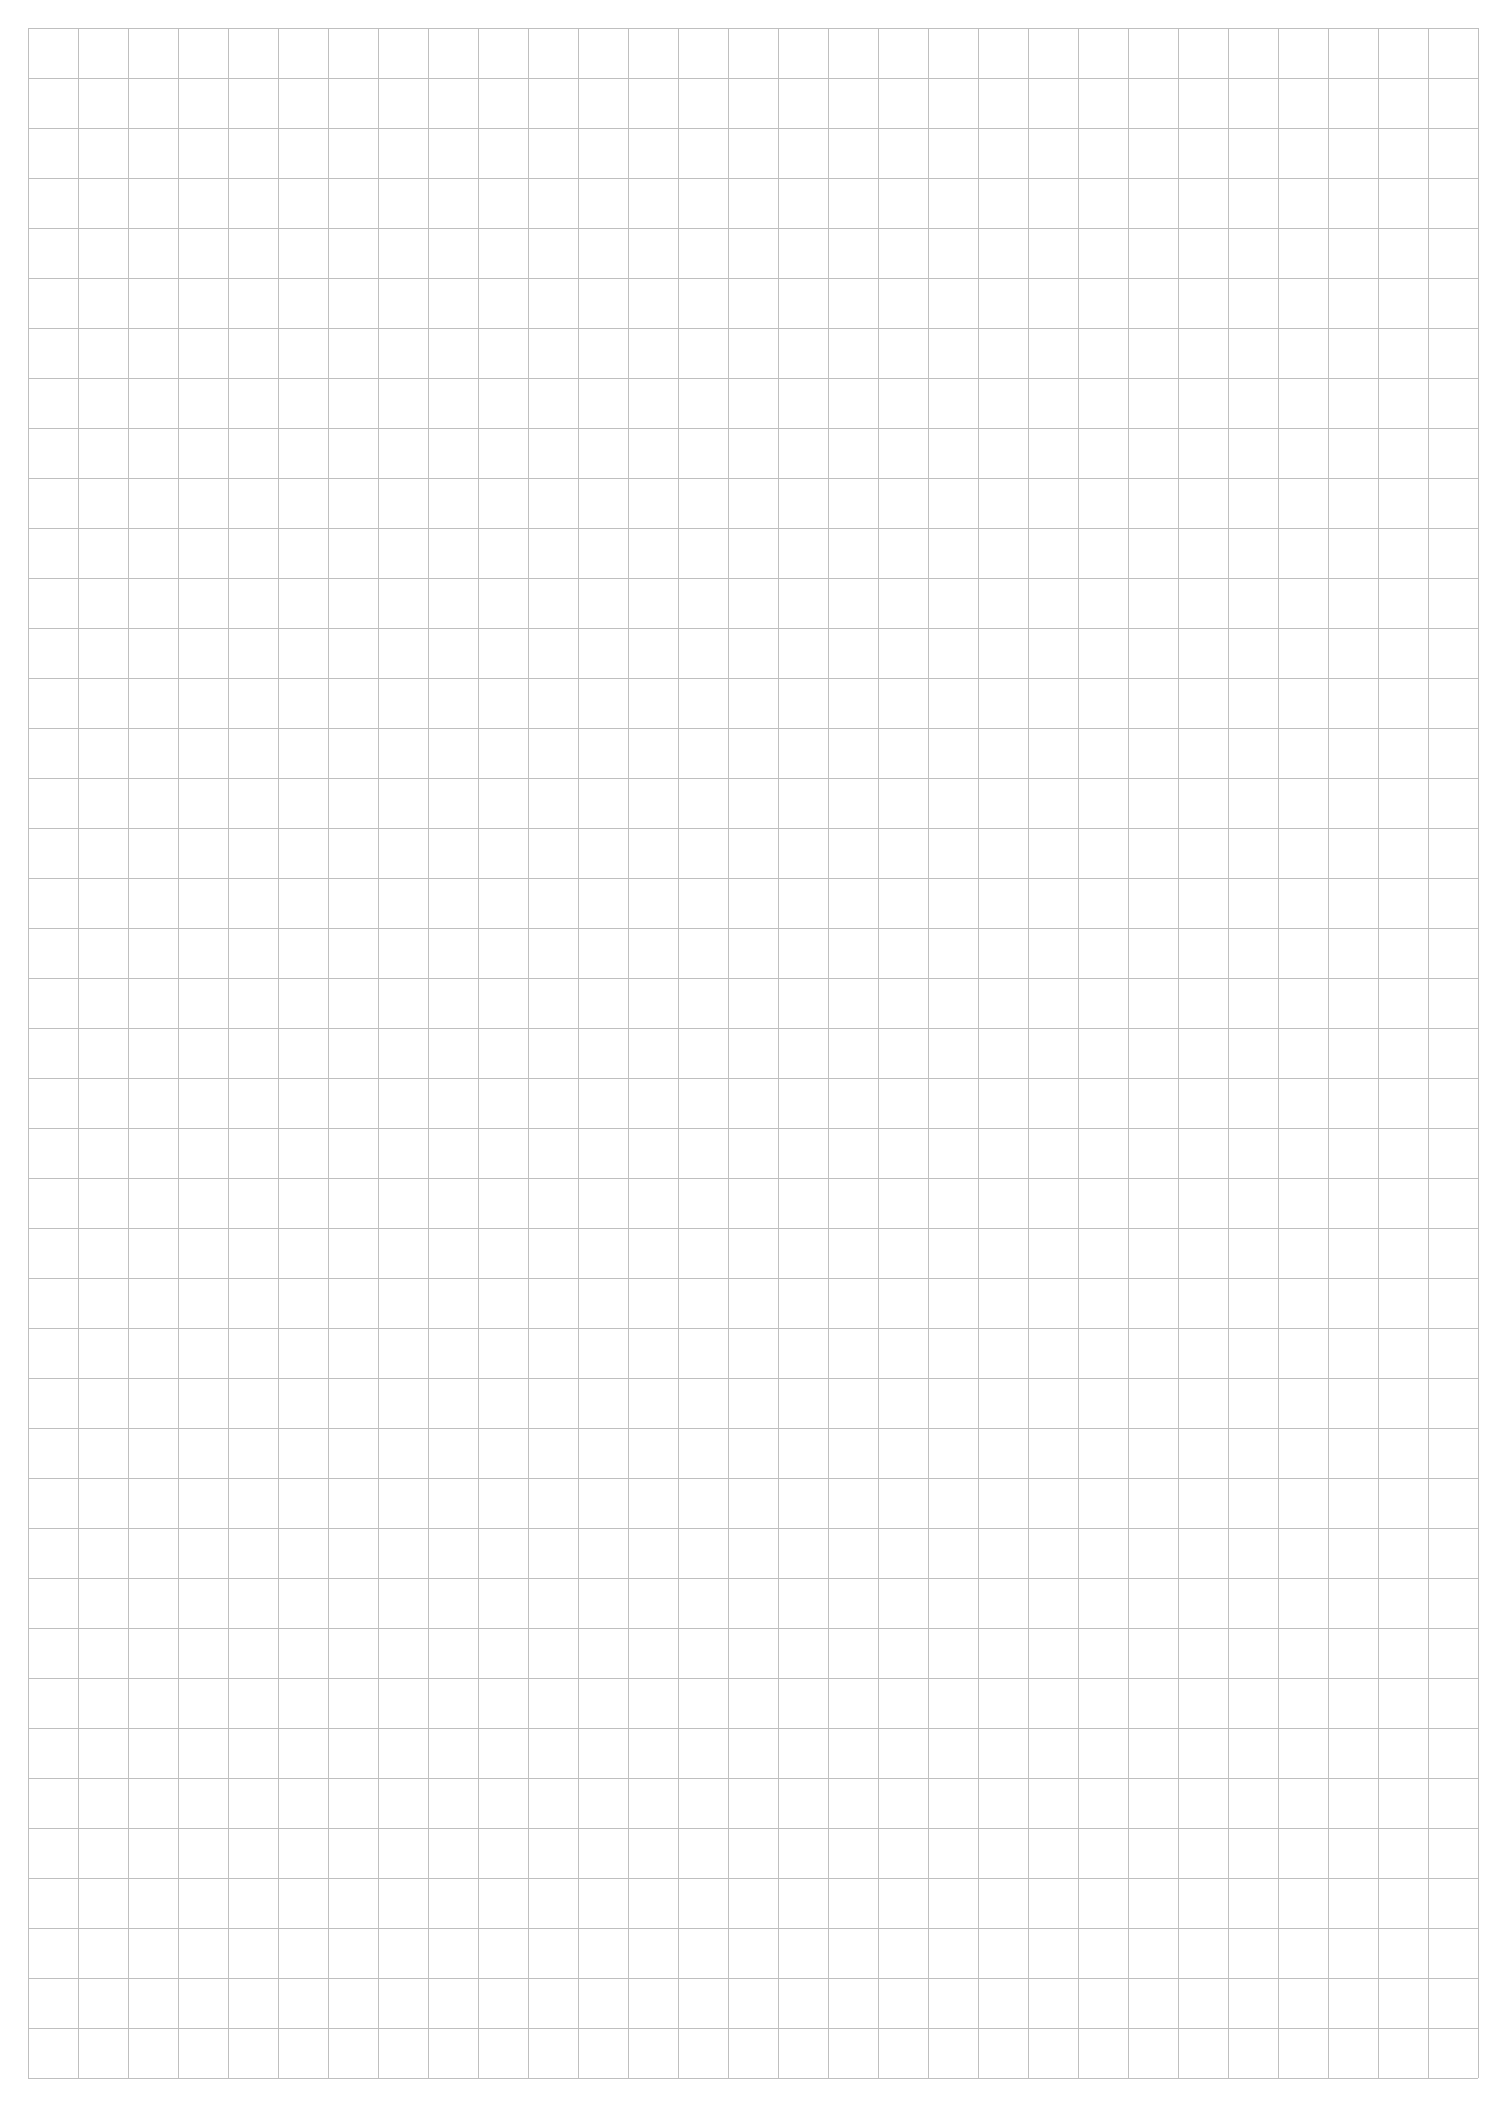
\begin{tikzpicture}[line width=0.1mm]
		\draw[color=gray!50, step=0.25in] (0,0) grid +(7.25in,10.25in);
	\end{tikzpicture}
\end{textblock*}

\begin{textblock*}{4in}(1in, 0.2in)
	\cbox{
		\underline{Exercise 2} \parm
		Jacques and Gilles are high-wire artistes. Gille weighs $780\,$N. How much does Jacques weigh?
		\begin{center}
			\tikz{%color
				
				\coordinate (J) at (2,0);
				\coordinate (A) at ($ (J)+(160:2) $);
				\coordinate (G) at ($ (J)+(-4:5) $);
				\coordinate (B) at ($ (G)+(16:2) $);
				\draw[thick] (A)--(J)--(G)--(B);
				\path ($ (current bounding box.south west)+(-0.5,-0.5) $) rectangle  ($ (current bounding box.north east)+(0.5,1.25) $);
				
				\node[below left] at (J) {J};
				\node[below right] at (G) {G};
				\node[below left] at (A) {A};
				\node[below right] at (B) {B};
				\draw[thin, gray] ($ (J)+(0,-0.25) $) -- +(0,-1);
				\draw[ultra thick, -latex] (G) -- +(0,-1.5) node[black, below,yshift=0.125cm] {\small $780\,$N};

				\draw[thin, {Latex[length=3pt]}-{Latex[length=3pt]}] ($ (J)+(0,-0.875) $) arc [start angle =-90, end angle=-4, radius = 0.875] node[fill=white, midway, inner sep=0.75mm] {\small $ 86\deg $};
				\draw[thin, {Latex[length=3pt]}-{Latex[length=3pt]}] ($ (J)+(0,-0.875) $) arc [start angle =270, end angle=160, radius = 0.875] node[fill=white, midway, inner sep=0.75mm] {\small $ 110\deg $};
				\draw[thin, {Latex[length=3pt]}-{Latex[length=3pt]}] ($ (G)+(0,-0.875) $) arc [start angle =-90, end angle=16, radius = 0.875] node[fill=white, midway, inner sep=0.75mm] {\small $ 106\deg $};
				\draw[thin, {Latex[length=3pt]}-{Latex[length=3pt]}] ($ (G)+(0,-0.875) $) arc [start angle =270, end angle=176, radius = 0.875] node[fill=white, midway, inner sep=0.75mm] {\small $ 94\deg $};
				% \draw[red, thin] (current bounding box.south west) rectangle (current bounding box.north east);
			}	

      
		
		\end{center}
	}
\end{textblock*}
\begin{textblock*}{2cm}(5.725cm, 5cm)
	\tikz{%color
		\coordinate (origin) at (0,0);
		\Skywalker[0.625]{origin}{Gray}{Gray}{Black}{white}{0.5}{.25}
	}
\end{textblock*}
\begin{textblock*}{2cm}(10.74cm, 5.325cm)
	\tikz{%color
		\coordinate (origin) at (0,0);
		\Skywalker[-0.75]{origin}{Gray}{Gray}{Black}{white}{0.55}{.25}
	}
\end{textblock*}
%%%%%%%%%%%%%%%%%%%%%%%%%%%%%%%%%%%%%%%%%%%%%%%%%%%%%%%%%%%%%%%%%%%%%%%%%%%%%%%%%%%%%%%%%%%%%%%%%%%%
% page 3
%%%%%%%%%%%%%%%%%%%%%%%%%%%%%%%%%%%%%%%%%%%%%%%%%%%%%%%%%%%%%%%%%%%%%%%%%%%%%%%%%%%%%%%%%%%%%%%%%%%%

.\newpage
\begin{textblock*}{7.25in}(1in, 0.4in)
	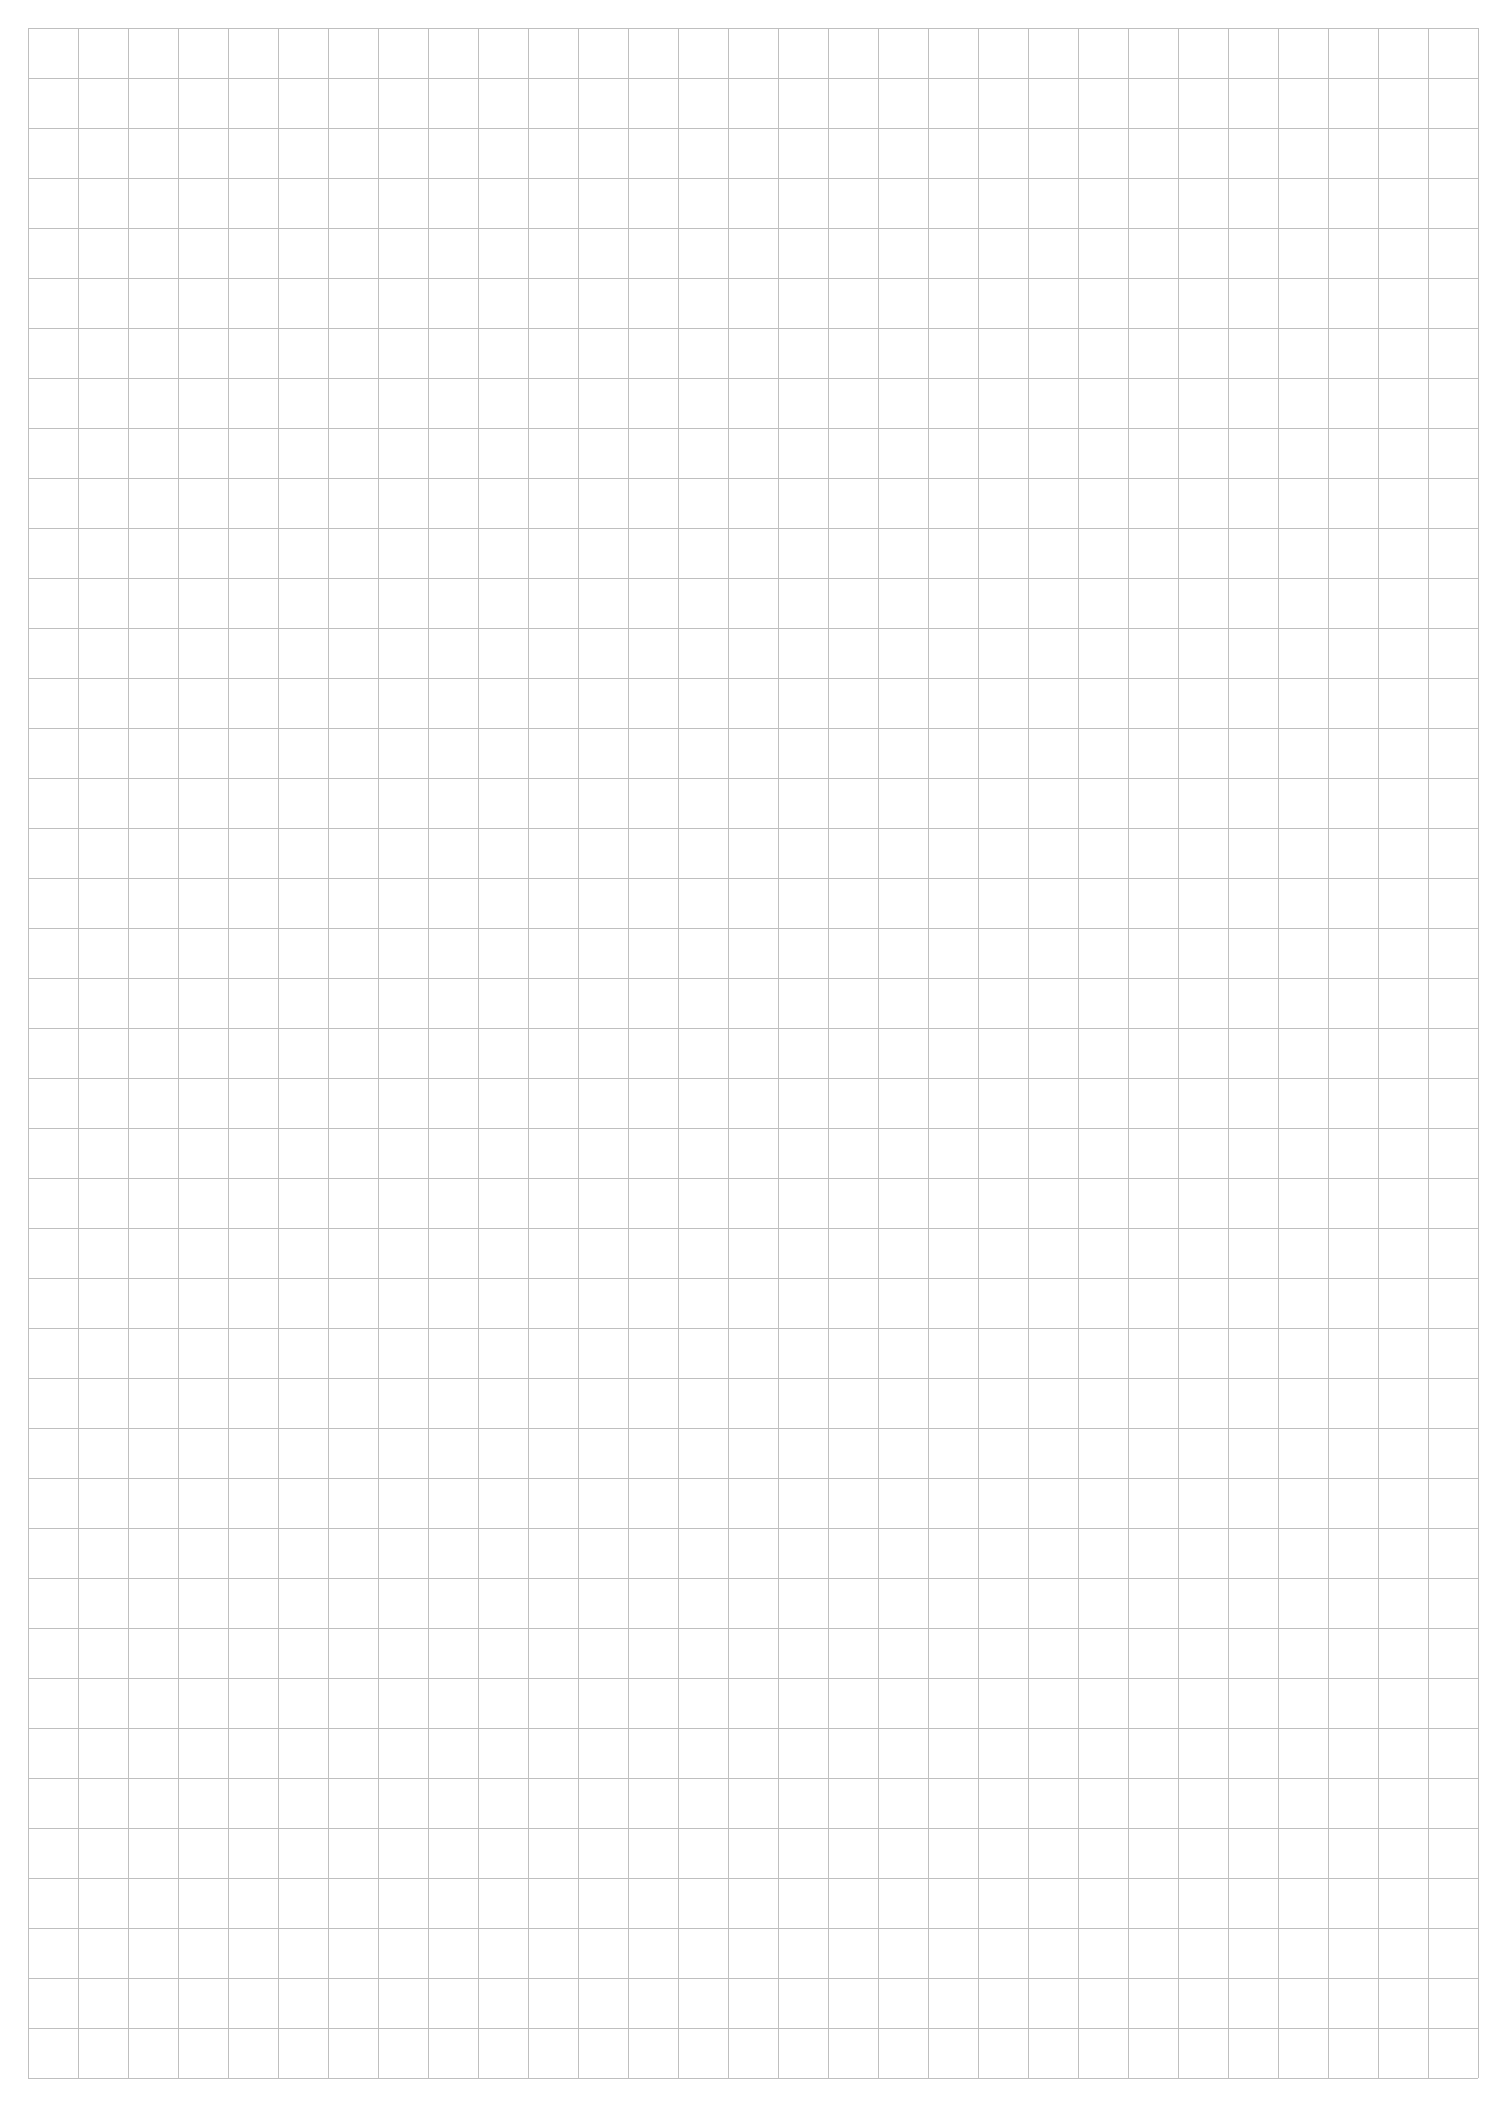
\begin{tikzpicture}[line width=0.1mm]
		\draw[color=gray!50, step=0.25in] (0,0) grid +(7.25in,10.25in);
	\end{tikzpicture}
\end{textblock*}

\begin{textblock*}{4in}(1in, 0.25in)
	\cbox{
		\underline{Example 3} \parm
		Determine the internal forces in members $AC$ and $BC$. \lb Specify whether they are in tension or compression.

	}
\end{textblock*}
\begin{textblock*}{2.25in}(5.525in, 0.25in)
	\cbox{
		\centering
		\scalebox{0.6}{
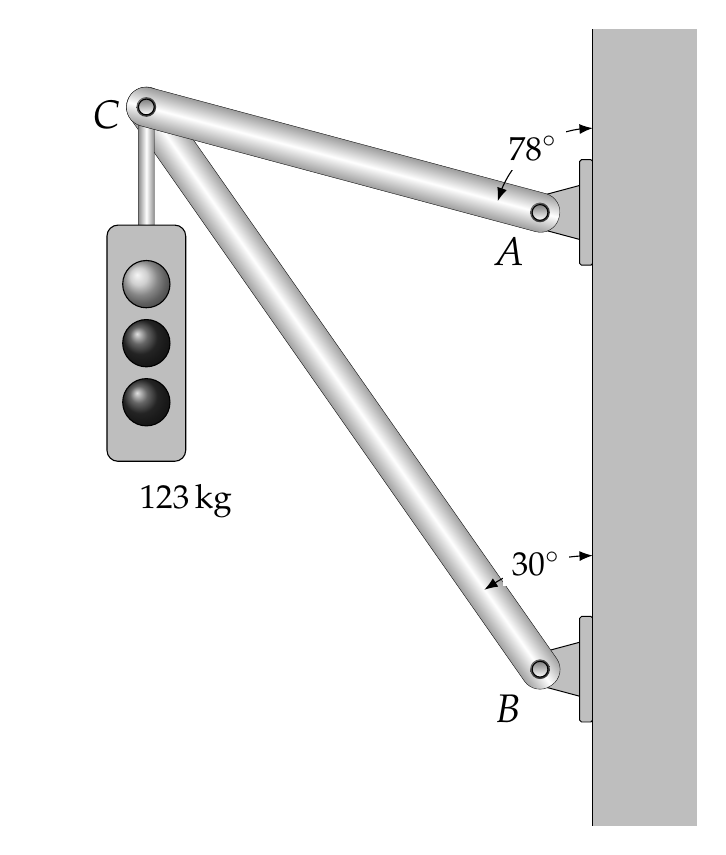
\begin{tikzpicture}

	\coordinate (C) at (0,0);
	\coordinate (B) at ($ (C)+(-15:5.176) $);
	\coordinate (A) at ($ (C)+(-55:8.717) $);
	\coordinate (D) at ($ (C)+(0,-3) $);

	\gettikzxy{(A)}{\ax}{\ay}
  \gettikzxy{(B)}{\bx}{\by}
  \gettikzxy{(C)}{\cx}{\cy}

	\PC[90]{B}{Gray!50}{black}{0.67}{0.125}
	\PC[90]{A}{Gray!50}{black}{0.67}{0.125}

	\fill[Gray0] ($ (\bx+0.67cm, \cy+1cm) $) rectangle ($ (\ax+2cm, \ay-2cm) $);
	\draw[thin]  ($ (\bx+0.67cm, \cy+1cm) $) -- ($ (\bx+0.67cm, \ay-2cm) $);
	
	\Meme{C}{A}{Gray}{White}{black}{0.5}{0.24}{0.125}	
	\Meme{C}{D}{Gray}{White}{black}{0.2}{.1}{0.125}
	\Meme{C}{B}{Gray}{White}{black}{0.5}{0.24}{0.125}

	\filldraw[rounded corners, fill=Gray0] ($ (D)+(-0.5,-1.5) $) rectangle ($ (D)+(0.5,1.5) $);
	\shadedraw[ball color=gray!40!black] (D) circle (.3cm);
	\shadedraw[ball color=gray!50] ($(D)+(0,0.75)$) circle (.3cm);
	\shadedraw[ball color=gray!40!black] ($(D)+(0,-0.75)$) circle (.3cm);
	\node at ($ (D)-(-0.5,2) $) {\large $ 123\,$kg};

	\draw[Latex-Latex] ($ (B)+(-15:0.6936)+(0,1.25) $) arc (90:165:1.25) node[midway,fill=white] {\large $78\deg$};
	\draw[Latex-Latex] ($ (A)+(-55:1.168)+(0,2.4) $) arc (90:125:2.4) node[midway,fill=white] { \large$30\deg$};

	\small
	
	\shadedraw [draw=black] (B) circle (0.1cm) node[ xshift=-0.4cm, yshift=-0.5cm] {\Large$A$};
	\shadedraw [draw=black] (A) circle (0.1cm) node[ xshift=-0.4cm, yshift=-0.5cm] {\Large$B$};
	\shadedraw [draw=black] (C) circle (0.1cm) node[ xshift=-0.5cm, yshift=-0.1cm] {\Large$C$};

	\pgfresetboundingbox
	\draw[white] (\cx-1.5cm, \cy+1cm) rectangle (\ax+2cm, \ay-2cm);
	

\end{tikzpicture}


}
		
	}
\end{textblock*}
\begin{textblock*}{3.5in}(1in, 6in)
	\cbox{
		\underline{Exercise 3} \parm
		Determine the internal forces in members $AC$ and $BC$. Specify whether they are in tension or compression.

	}
\end{textblock*}
\begin{textblock*}{2.75in}(5.025in, 6in)
	\cbox{
		\centering
	
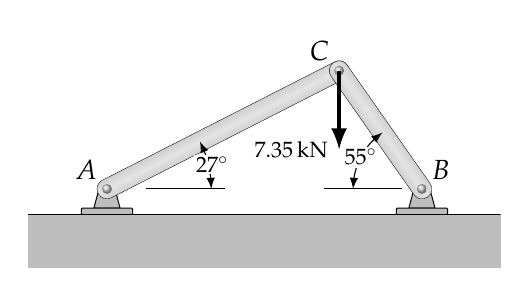
\begin{tikzpicture}

	\coordinate (A) at (-2,0);
	\coordinate (AA) at ($ (A)+(27:4) $);
	\coordinate (B) at (2,0);
	\coordinate (BB) at ($ (B)+(125:2.5) $);
	\path[name path=AC] (A)--(AA);
	\path[name path=BC] (B)--(BB);
	\path[name intersections = {of=AC and BC, by=C}];

	\PC{A}{Gray0}{black}{0.325}{0.125}
	\PC{B}{Gray0}{black}{0.325}{0.125}
	\fill[Gray0] ($ (A)+(-1,-0.325) $) rectangle ($ (B)+(1,-1) $);
	\draw ($ (A)+(-1,-0.325) $) rectangle ($ (B)+(1,-0.325) $);
	\Meme{A}{C}{LightGrey}{LightGrey!50}{black}{0.25}{0.12}{0.125}
	\Meme{B}{C}{LightGrey}{LightGrey!50}{black}{0.25}{0.12}{0.125}
	\draw[ultra thick, -latex] (C) -- +(0,-1) node[left]{\footnotesize $7.35\,$kN};
	\node[above left] at (C) {$ C $};
	\node[above left] at (A) {$ A $};
	\node[above right] at (B) {$ B $};

	\draw[thin] ($ (B)-(.25,0) $) -- +(-1,0);
	\draw[thin] ($ (A)+(.5,0) $) -- +(1,0);

	\draw[latex-latex] ($ (A)+(0:1.325) $) arc (0:27:1.325) node[midway, fill=white, inner sep=0.2mm, xshift=0.5mm] {\footnotesize $27\deg$};
	\draw[latex-latex] ($ (B)+(125:0.875) $) arc (125:180:0.875) node[midway, fill=white, inner sep=0.3mm] {\footnotesize $55\deg$};

	%  \Meme{A}{B}{Black}{White}{Red}{0.25}{0.125}{0.125}





	
	% \draw (current bounding box.south west) rectangle (current bounding box.north east);

	

\end{tikzpicture}



		
	}
\end{textblock*}

%%%%%%%%%%%%%%%%%%%%%%%%%%%%%%%%%%%%%%%%%%%%%%%%%%%%%%%%%%%%%%%%%%%%%%%%%%%%%%%%%%%%%%%%%%%%%%%%%%%%
% page 4
%%%%%%%%%%%%%%%%%%%%%%%%%%%%%%%%%%%%%%%%%%%%%%%%%%%%%%%%%%%%%%%%%%%%%%%%%%%%%%%%%%%%%%%%%%%%%%%%%%%%
.\newpage
\begin{textblock*}{7.25in}(1in, 0.4in)
	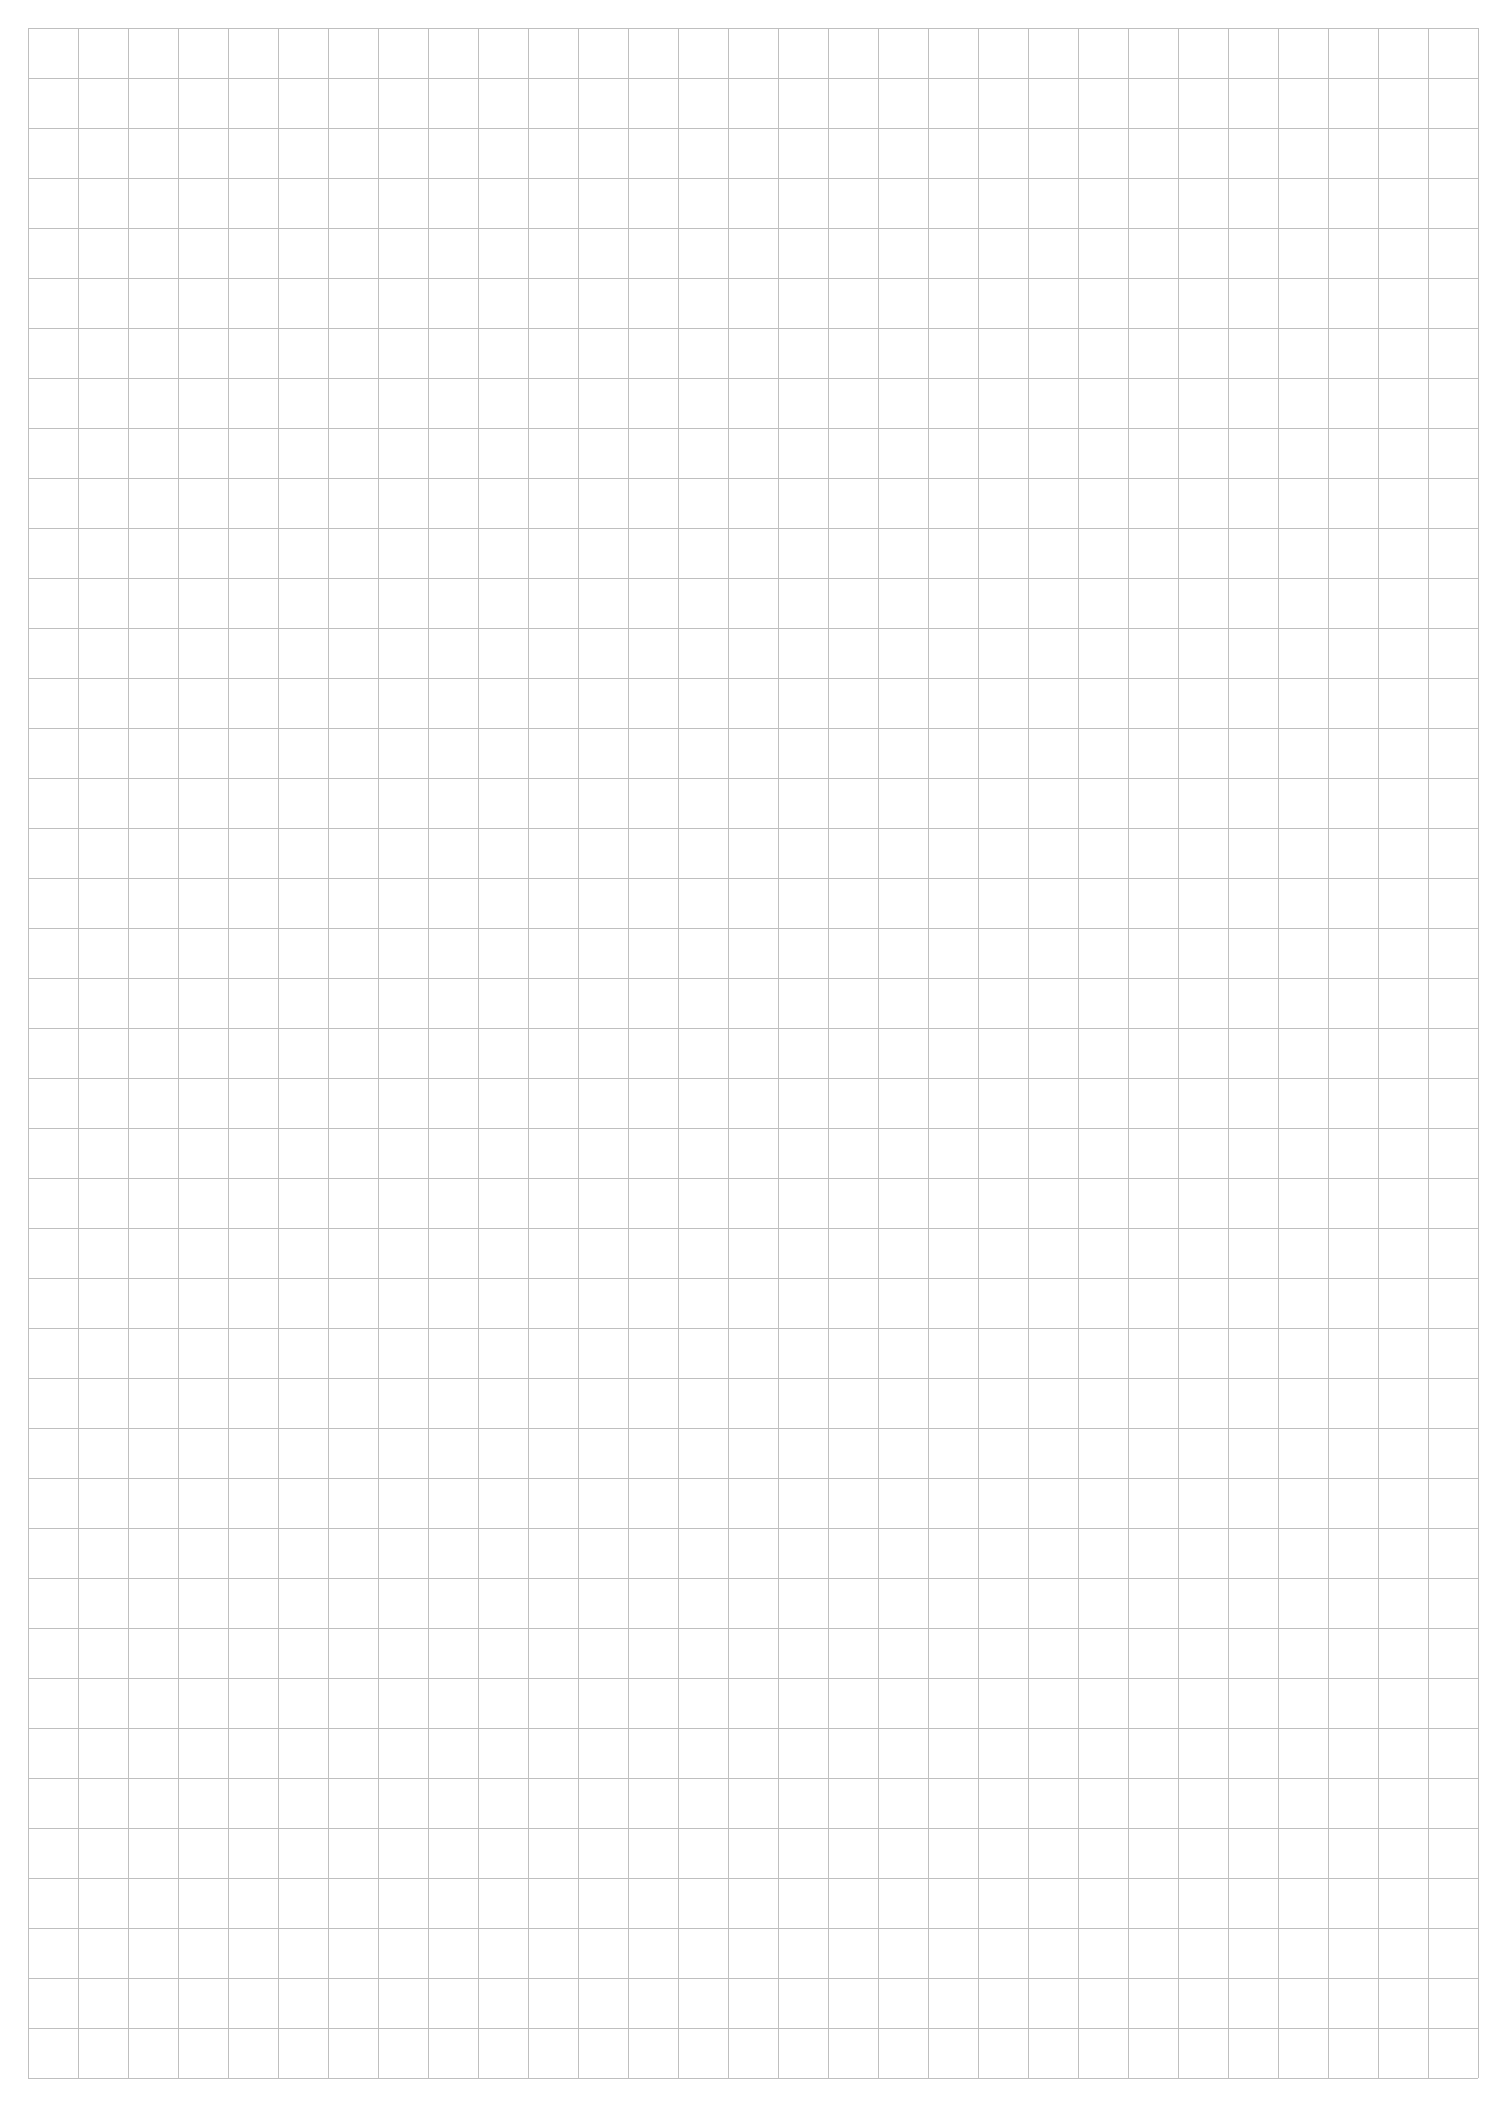
\begin{tikzpicture}[line width=0.1mm]
		\draw[color=gray!50, step=0.25in] (0,0) grid +(7.25in,10.25in);
	\end{tikzpicture}
\end{textblock*}

\begin{textblock*}{3in}(1in, 0.2in)
	\cbox{
		\underline{Example 4} \parm
		Determine $\theta$. Then find the tension in the rope and the pulley
		reaction at $B$ due to the suspended mass.

	}
\end{textblock*}
\begin{textblock*}{3.25in}(4.525in, 0.2in)
	\cbox{
		\centering
		\def\scale{0.8}
		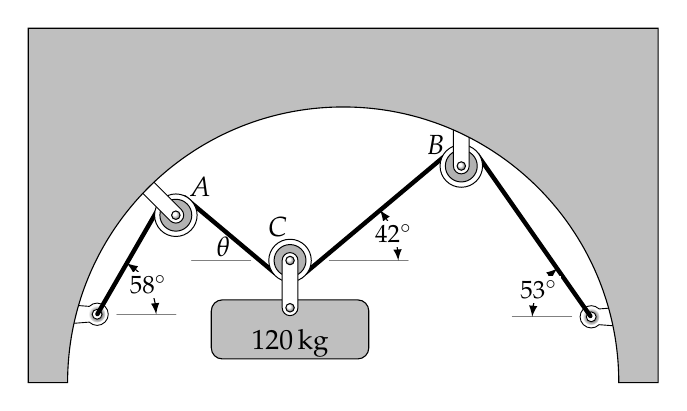
\begin{tikzpicture}[line cap=round]

  \coordinate (A) at (-2.125,2.125);
  \coordinate (B) at (1.5,2.75);
  \coordinate (C) at (-0.675,1.55);
  \coordinate (AA) at (-3.125,0.8675);
  \coordinate (BB) at (3.15,0.835);
  \coordinate (Cright) at ($ (C)+(0.375, 0) $);
  \coordinate (Cleft) at ($ (C)+(-0.375, 0) $);

 \filldraw[fill=Gray!50, rounded corners] ($ (C)+(-1,-.5) $) rectangle +(2,-0.75);
  \EyeBolt[-90]{AA}{White}{black}{0.5}{0.325}
  \EyeBolt[90]{BB}{White}{black}{0.5}{0.325}
  \draw[black, ultra thick] ($ (C)+(-40:0.25) $) -- +(40:2.3);
  \draw[black, ultra thick] ($ (C)+(220:0.25) $) -- +(140:1.5);
  \draw[black, ultra thick] ($ (A)+(170:0.25) $) -- +(240:1.5);
  \draw[black, ultra thick] ($ (B)+(35:0.25) $) -- +(-55:2.5);
  \PulleyC[225]{A}{White}{Black}{1.5}{0.25}{0.4}{0.125}
  \PulleyC[180]{B}{White}{Black}{1.5}{0.25}{0.4}{0.125}
  \PulleyC{C}{White}{Black}{1.5}{0.25}{0.4}{0.125}
  \filldraw[fill=Gray!50] (-4,0)-- +(0.5,0)arc(180:90:3.5)arc(90:0:3.5) -- (4,0) -- ++(0,4.5) -- ++(-8,0) -- cycle;
  \node at ($ (C)+(0,-0.75) $) [below] {$ 120\,$kg};
  \draw[thin, gray] ($ (C)+(0.5,0) $) -- +(1,0);
  \draw[thin, gray] ($ (C)+(-0.5,0) $) -- +(-0.75,0);
  \draw[thin, gray] ($ (BB)+(-0.25,0) $) -- +(-0.75,0);
  \draw[thin, gray] ($ (AA)+(0.25,0) $) -- +(0.75,0);
  \draw[latex-latex] ($ (Cright)+(1,0) $) arc (0:40:1) node[midway, fill=white, inner sep=0.5mm] {\small$42\deg$};
  \node at ($ (C)+(110:0.45) $) {$C$};
  \node at ($ (B)+(140:0.425) $) {$B$};
  \node at ($ (A)+(50:0.475) $) {$A$};
  \node at ($ (Cleft)+(160:0.5) $) {$\theta$};
  \draw[latex-latex] ($ (AA)+(0.75,0) $) arc (0:60:0.75) node[midway, fill=white, inner sep=0.5mm] {\small$58\deg$};
  \draw[latex-latex] ($ (BB)-(0.75,0) $) arc (180:125:0.75) node[midway, fill=white, inner sep=0.5mm] {\small$53\deg$};

  % \fill[green] (Cright) circle (0.5mm);


\end{tikzpicture}
	}
\end{textblock*}

%%%%%%%%%%%%%%%%%%%%%%%%%%%%%%%%%%%%%%%%%%%%%%%%%%%%%%%%%%%%%%%%%%%%%%%%%%%%%%%%%%%%%%%%%%%%%%%%%%%%
% page 5
%%%%%%%%%%%%%%%%%%%%%%%%%%%%%%%%%%%%%%%%%%%%%%%%%%%%%%%%%%%%%%%%%%%%%%%%%%%%%%%%%%%%%%%%%%%%%%%%%%%%
~\newpage
\begin{textblock*}{7.25in}(1in, 0.4in)
	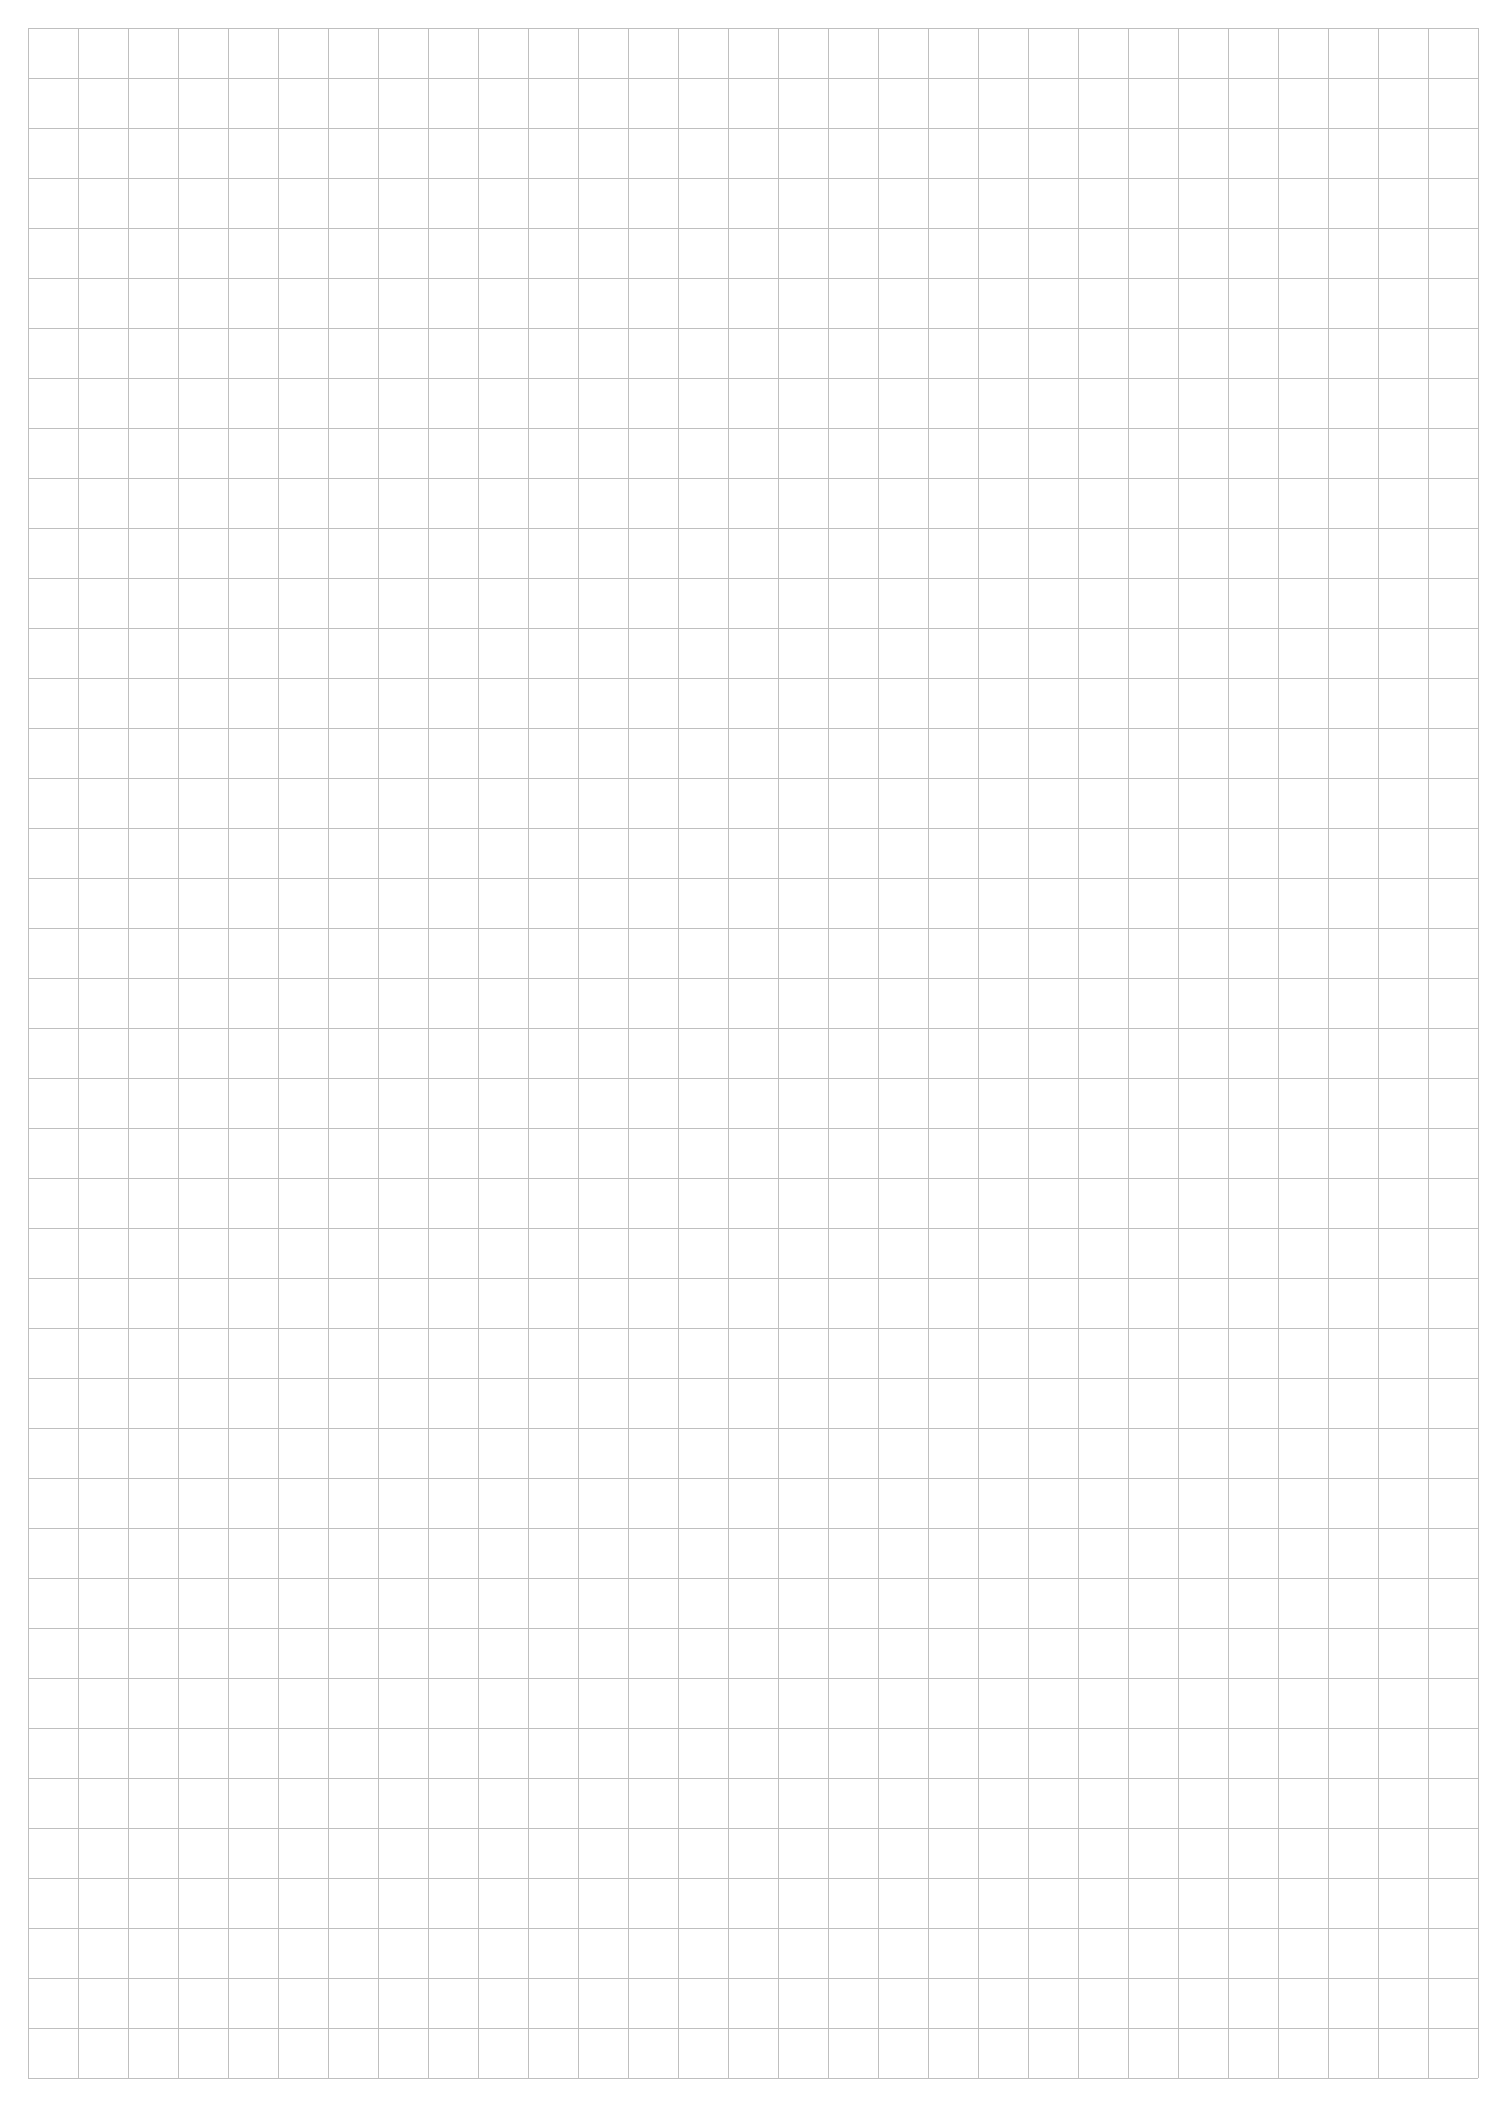
\begin{tikzpicture}[line width=0.1mm]
		\draw[color=gray!50, step=0.25in] (0,0) grid +(7.25in,10.25in);
	\end{tikzpicture}
\end{textblock*}


\begin{textblock*}{3in}(1in, 0.2in)
	\cbox{
		\underline{Exercise 4} \parm
		Cylinder $B$ has a mass of 28 kg. The system is in equilibrium.
		Determine the mass of $A$ and the reactions at $C$ and $E$.

	}
\end{textblock*}
\begin{textblock*}{3.25in}(4.525in, 0.2in)
	\cbox{
		\centering
		\def\scale{0.8}
		% !TEX root = ../../Beamer/03EquilibriumOfAParticle/03Equilibrium.tex

\tikz[line cap=round, scale=0.9]{
	\coordinate (A) at (0,-2);
	\coordinate (B) at (0,0);
	\coordinate (C) at (-3,0);
	\coordinate (D) at ($ (30:3.746)+(-60:0.25) $);
	\coordinate (E) at ($ (D)+(0.2625,0)+(0,-2.5) $);

	\fill[right color=Gray, left color=Gray!50] ($ (C)+(-0.5,-1.5) $) rectangle +(-0.75,3);
	\fill[bottom color=Gray, top color=Gray!50] ($ (D)+(-1.5,.5) $) rectangle +(3,0.75);

	\EyeConnection[-90]{C}{Gray!50}{black}{0.5}{0.5}
	\Ring{B}{Gray!50}{Gray}{.25}{0.125}{0.01};

	\draw[ultra thick, Black] ($ (B)+(30:0.1) $) -- ++(30:3.646)arc(120:0:0.25)-- ++(0,-2.5);
	\draw[ultra thick, Black]($ (B)+(180:0.1) $) -- ($ (C)+(0.025,0) $);
	\draw[ultra thick, Black]($ (B)+(270:0.1) $) -- ++(0,-2);
	\Pulley[180]{D}{Gray0}{black}{0.5}{0.125}
	\draw[left color=Gray, right color=Gray, middle color=Gray!30] ($(A)+(-0.5,-.75)$) rectangle ($(A)+(0.5,0.75)$);
	\draw[left color=Gray, right color=Gray, middle color=Gray!30] ($(E)+(-0.5,-.75)$) rectangle ($(E)+(0.5,0.75)$);
	\draw[thin] ($ (B)+(0.5,0) $) -- +(1.5,0)node[right]{$ x $};
	\draw[latex-latex] ($ (B)+(1.5,0) $)arc(0:30:1.5)node[midway, fill=white, inner sep=0.25mm]{$ 32^\circ $};
	\node at (A) {\Large $A$};
	\node at (E) {\Large $B$};
	\node[yshift=0.5cm] at (C) {\Large $C$};
	\node[xshift=0.5cm] at (D) {\Large $E$};
	\node[xshift=-0.325cm, yshift=0.325cm] at (B) {\Large $D$};
	\node[ yshift=-1cm] at (E) {\large $28\,\text{kg}$};
}

	}
\end{textblock*}



%%%%%%%%%%%%%%%%%%%%%%%%%%%%%%%%%%%%%%%%%%%%%%%%%%%%%%%%%%%%%%%%%%%%%%%%%%%%%%%%%%%%%%%%%%%%%%%%%%%%
% page 6
%%%%%%%%%%%%%%%%%%%%%%%%%%%%%%%%%%%%%%%%%%%%%%%%%%%%%%%%%%%%%%%%%%%%%%%%%%%%%%%%%%%%%%%%%%%%%%%%%%%%
~\newpage
\begin{textblock*}{7.25in}(1in, 0.4in)
  % \textblockcolor{pink}
	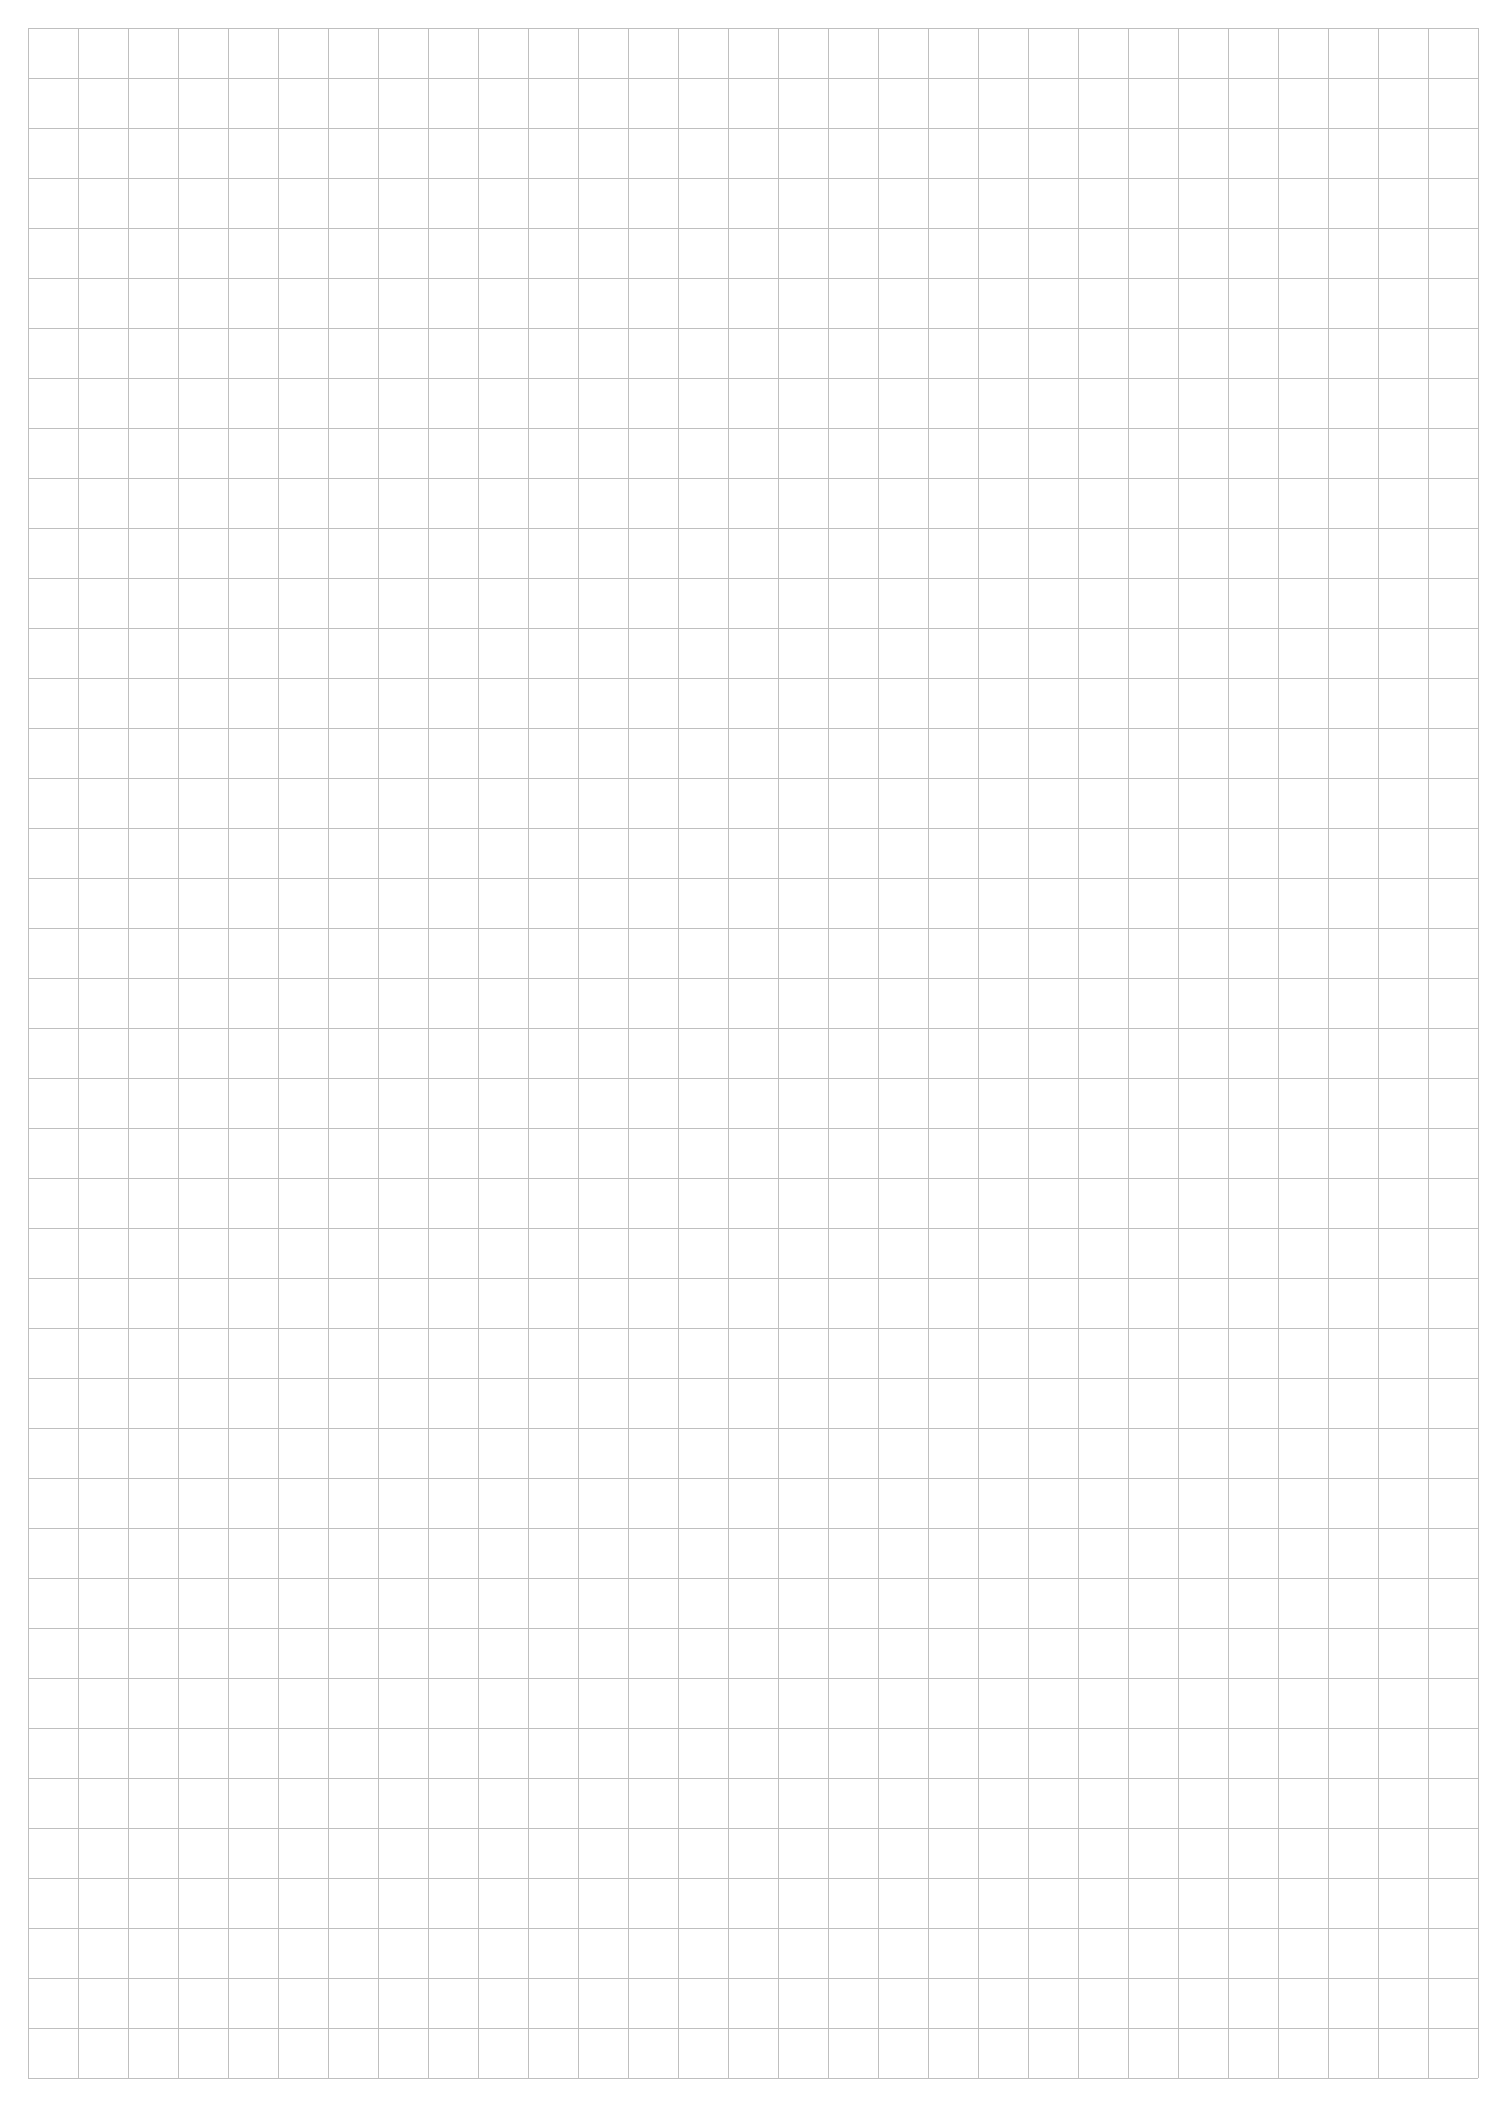
\begin{tikzpicture}[line width=0.1mm]
		\draw[color=gray!50, step=0.25in] (0,0) grid +(7.25in,10.25in);
	\end{tikzpicture}
\end{textblock*}

\begin{textblock*}{3in}(1in, 0.2in)
	\cbox{
		\underline{Example 5} \parm
		Determine the maximum weight $W$ of the bucket that the system can support given that no single wire may support more than $450\,$N. Determine $R_C$, the reaction at $C$, for this value of $W$.

	}
\end{textblock*}
\begin{textblock*}{3.25in}(4.525in, 0.2in)
	\cbox{
		\centering
		\def\scale{0.8}
		% !TEX root = ../../Beamer/03EquilibriumOfAParticle/03Equilibrium.tex

\tikz[line cap=round, scale=\scale]{
	\coordinate (A) at (0,0);
	\coordinate (B) at (2,0);
	\coordinate (C) at (6,2);
	\coordinate (D) at (4,-2);
	\coordinate (E) at (4,-3.5);





  \Ring{B}{LightGrey}{LightGrey}{0.25}{0.125}{0.02}
  \Ring{D}{LightGrey}{LightGrey}{0.25}{0.125}{0.02}

  \EyeConnection[-90]{A}{LightGrey!50}{black}{0.75}{0.5}
  \EyeConnection[90]{C}{LightGrey!50}{black}{0.75}{0.5}

  \draw[ultra thick, Black] ($(B)+(0.05,-0.05)$) -- ($(D)+(-0.05,0.05)$);
  \draw[ultra thick, Black] ($(A)+(0.05,0)$) -- ($(B)+(-0.0875,0)$);
  \draw[ultra thick, Black] ($(B)+(30:0.05)$) -- ($(C)+(210:0.05)$);
  \draw[ultra thick, Black] ($(D)+(63:0.05)$) -- ($(C)+(243:0.05)$);
  \draw[ultra thick, Black] ($(D)+(0,-0.05)$) -- +(0,-1);

	\filldraw[left color=LightGrey, right color=LightGrey, middle color=LightGrey!5] (E)-- ++(-0.5,0)-- ++(0.25,-1)-- ++(0.5,0)-- ++(0.25,1) -- cycle;

	\draw[thick] ($(E)+(0.5,0)$)arc(0:180:0.5);

  \fill[left color=LightGrey!40, right color=LightGrey] ($(A)+(-0.25,1)$) rectangle ($(A)+(-1,-2)$);
	\draw ($(A)+(-0.25,1)$) rectangle ($(A)+(-0.25,-2)$);
  \fill[right color=LightGrey!40, left color=LightGrey] ($(C)+(0.25,1)$) rectangle ($(C)+(1,-2)$);
	\draw ($(C)+(0.25,1)$) rectangle ($(C)+(0.25,-2)$);

  \node[below right] at (A) {$A$};
  \node[xshift=-0.325cm, yshift=0.325cm] at (B) {$B$};
  \node[xshift=-0.325cm,yshift=0.325cm] at (C) {$C$};
  \node[xshift=-0.325cm,yshift=-0.325cm] at (D) {$D$};
  \node[yshift=-0.5cm] at (E) {$W$};

  \draw[thin] ($(B)+(0.5,0)$) -- +(2,0);
  \draw[thin] ($(D)+(0.5,0)$) -- +(2,0);

\small
  \draw[latex-latex] ($(B)+(2,0)$)arc(0:26.565:2)node[midway, fill=white, inner sep=0.5mm]{$25^\circ$};
  \draw[latex-latex] ($(B)+(2,0)$)arc(0:-45:2)node[midway, fill=white, outer sep=1mm]{$45^\circ$};
  \draw[latex-latex] ($(D)+(1.5,0)$)arc(0:63.46:1.5)node[midway, fill=white, outer sep=1mm]{$60^\circ$};

}

	}
\end{textblock*}







%%%%%%%%%%%%%%%%%%%%%%%%%%%%%%%%%%%%%%%%%%%%%%%%%%%%%%%%%%%%%%%%%%%%%%%%%%%%%%%%%%%%%%%%%%%%%%%%%%%%
% page 5
%%%%%%%%%%%%%%%%%%%%%%%%%%%%%%%%%%%%%%%%%%%%%%%%%%%%%%%%%%%%%%%%%%%%%%%%%%%%%%%%%%%%%%%%%%%%%%%%%%%%
.\newpage

\begin{textblock*}{7.25in}(1in, 0.4in)
  % \textblockcolor{pink}
	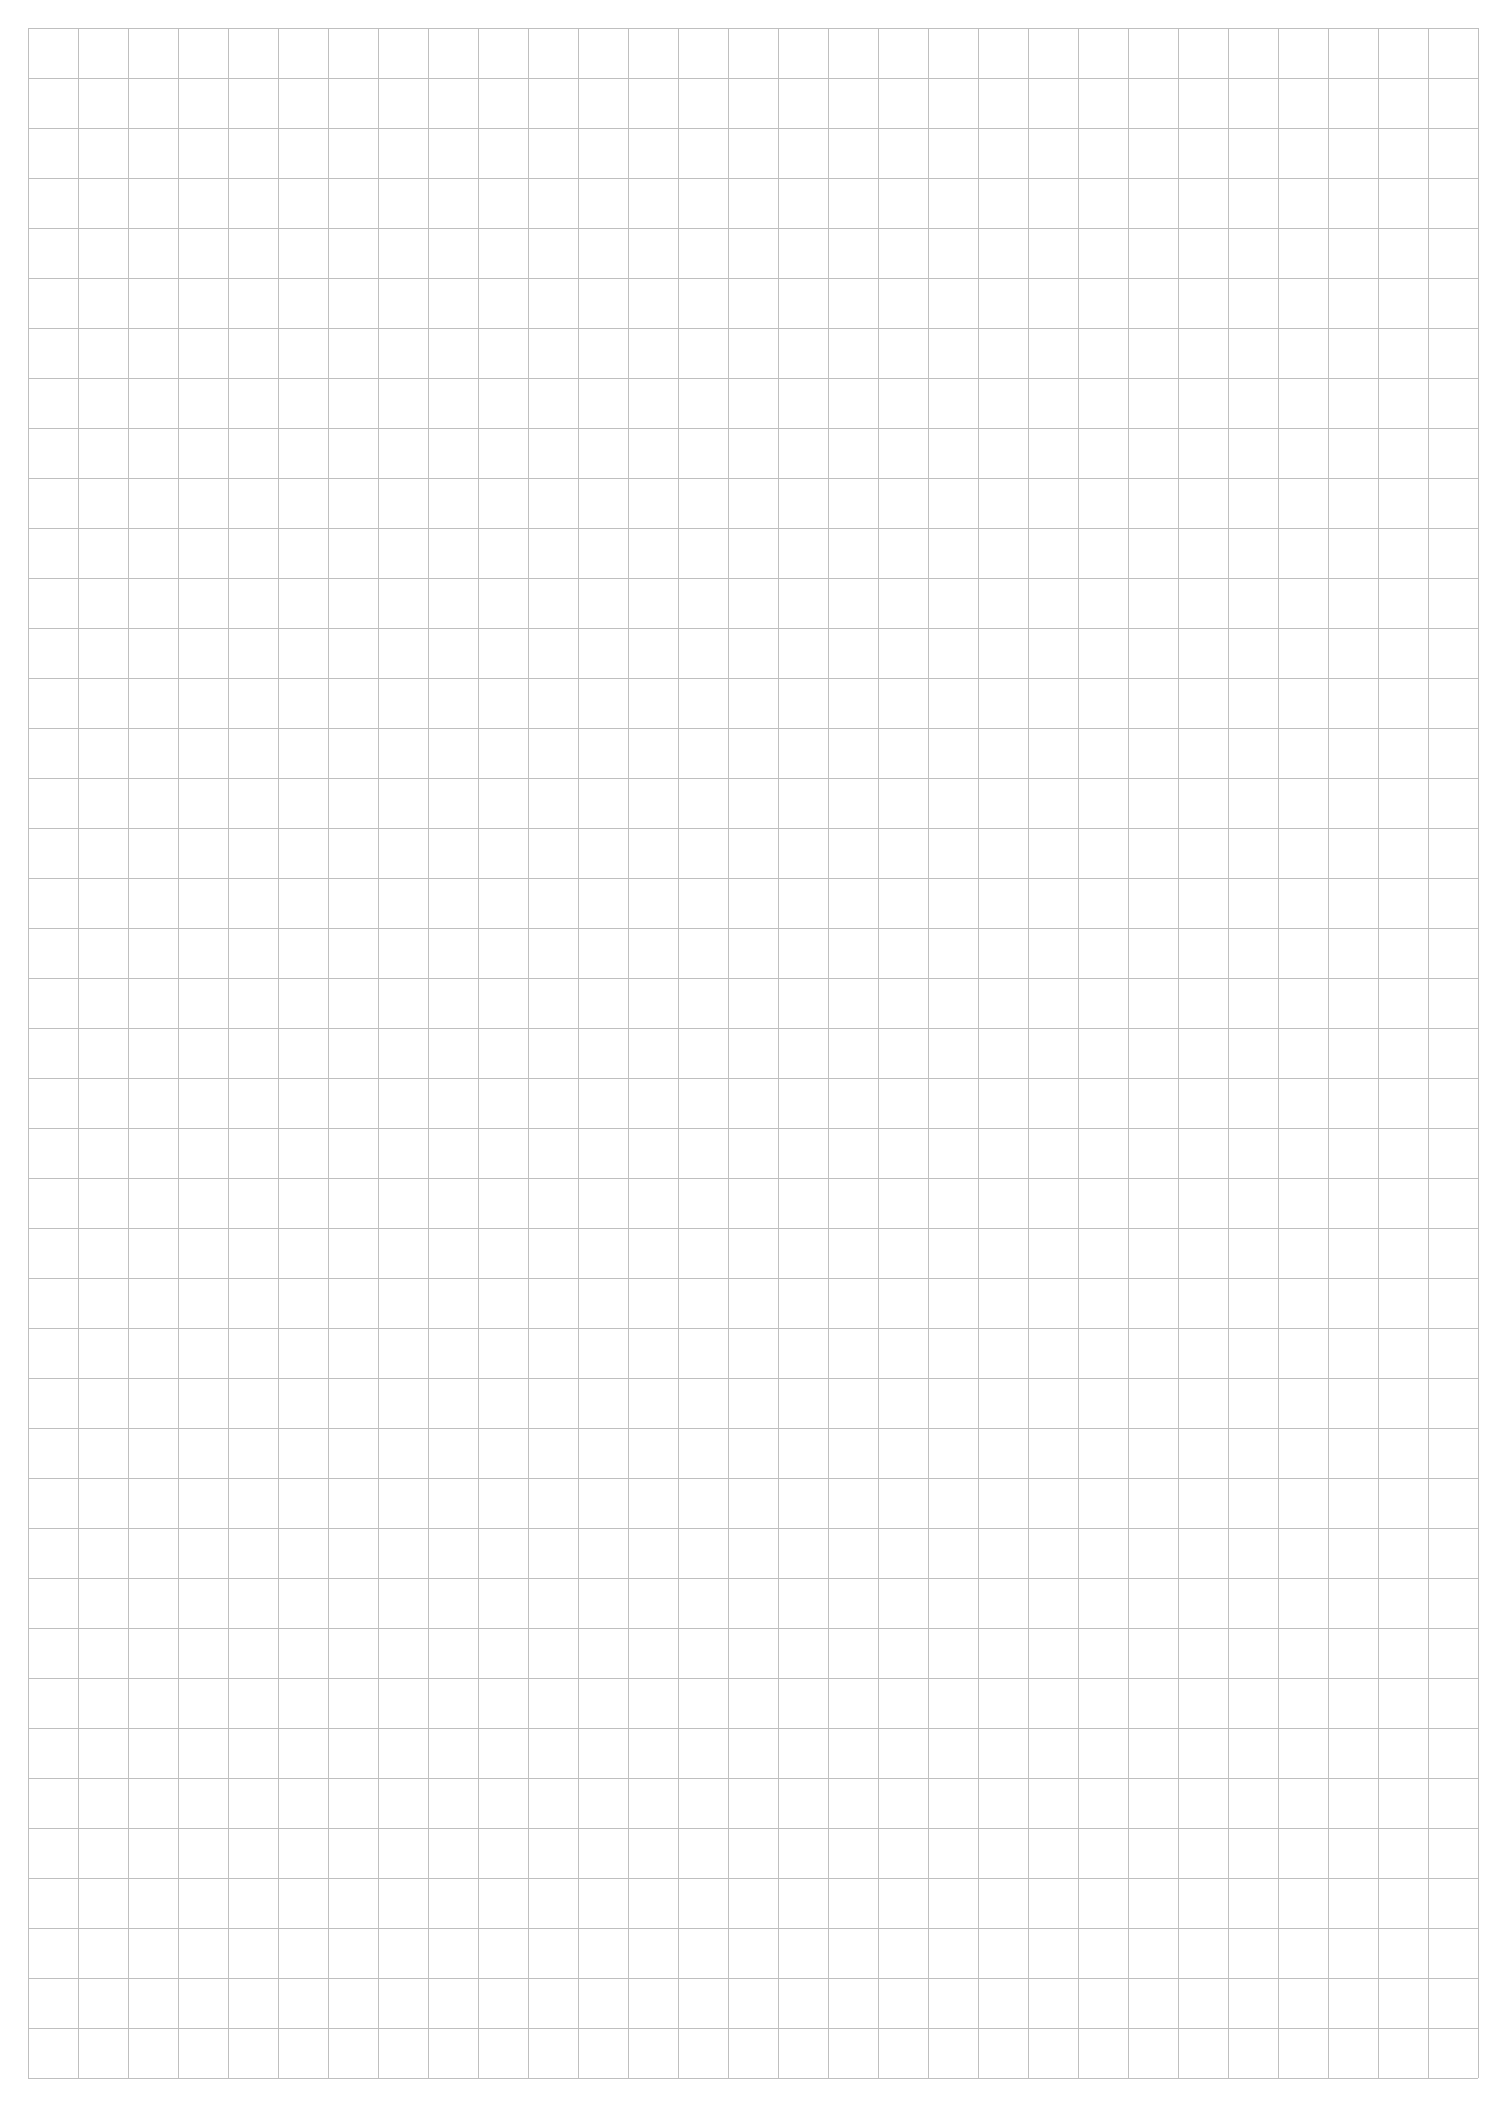
\begin{tikzpicture}[line width=0.1mm]
		\draw[color=gray!50, step=0.25in] (0,0) grid +(7.25in,10.25in);
	\end{tikzpicture}
\end{textblock*}
\begin{textblock*}{3.1275in}(1in, 0.225in)
	\cbox{
		\underline{Exercise 5} \parm
		The tension in cable $AC$ is $400\,$N. Determine the force $F$ necessary to hold the ring $A$ in the position shown..

	}
\end{textblock*}
\begin{textblock*}{3.125in}(4.65in, 0.225in)
	
	\cbox{
		\centering
		\def\scale{0.7}		
		\input{../../pikz/03EquiConcurrent/03EquiConc10Handout.tex}
	}
\end{textblock*}



\end{document}